

 \documentclass[oneside,11pt]{Classes/CUEDthesisPSnPDF}




\degree{Doctor of Philosophy}
\degreedate{July 2017}


\hbadness=10000
\hfuzz=5pt

% Put all the style files you want in the directory StyleFiles and usepackage like this:

%\usepackage{StyleFiles/watermark}
\usepackage{watermark}
\usepackage{amsmath,amsfonts,amssymb,amsthm,epsfig,epstopdf}
\usepackage[version=3]{mhchem}
\usepackage{xcolor}
\usepackage{caption}
\usepackage{booktabs}
\usepackage{nomencl}
\usepackage{natbib}
\usepackage{etoolbox}
\usepackage{cases}
\usepackage{longtable}
\usepackage{enumerate}
\usepackage{enumitem}
\usepackage{pdfpages}
\usepackage{graphicx}
\usepackage{float}
\usepackage{algorithm}
\usepackage{algpseudocode}
\usepackage[english]{babel}
\usepackage{subcaption}

%titling,url,array}

\theoremstyle{definition}
\newtheorem{defn}{Definition}[section]
\newtheorem{conj}{Conjecture}[section]
\newtheorem{exmp}{Example}[section]
\newtheorem{theorem}{Theorem}[section]
\newtheorem{corollary}{Corollary}[theorem]
\newtheorem{lemma}[theorem]{Lemma}
\newtheorem{remark}[theorem]{Remark}

\begin{document}
%\maketitle

\begin{titlepage}
	\begin{center}
	
	\begin{large}
	Annual Progress Seminar - I Report\\ on\\
	\end{large}			
		 
		
		\vspace*{1\baselineskip}
		\begin{huge}
			
		Social Network Analytics: Determining latent characteristics in data\\
		\end{huge}
			
		\vspace*{1\baselineskip}
		Submitted\\
in partial fulfillment of\\
the requirements of the degree of\\
\vspace*{1\baselineskip}
		\begin{large}
		Doctor of Philosophy (Computer Engineering) \\
		\end{large}
		\vspace*{1\baselineskip}
		
		by\\
		\vspace*{1\baselineskip}
		\begin{large}
			Pranav Nerurkar\\ 
		\end{large}
		(169070001)\\
		2016 - 2017\\
		\vspace*{1\baselineskip}
		Under Guidance Of\\
		\vspace*{1\baselineskip}
		\begin{large}
Dr. S. G. Bhirud (Guide)\\
Dr. M. M. Chandane (Co - Guide)\\
\end{large}
		
		
	\end{center}


\begin{center}
\includegraphics[scale=0.3]{VJTIM.jpg}\end{center}
\vspace*{1\baselineskip}

\begin{center}
\begin{Large}
Department of Computer Engineering \& Information Technology\\
Veermata Jijabai Technological Institute, Mumbai - 400019\\  
(Autonomous Institute Affiliated to University of Mumbai)\\
2016 - 2017
\end{Large}
\end{center}
\end{titlepage}

%set the number of sectioning levels that get number and appear in the contents
\setcounter{secnumdepth}{3}
\setcounter{tocdepth}{3}
\renewcommand{\chaptermark}[1]{\markboth{#1}{}}
\renewcommand{\sectionmark}[1]{\markright{#1}{}}
\rhead{} \chead{} \lhead{\leftmark} \rfoot{\footnotesize \thepage} \cfoot{} \lfoot{\footnotesize  \begin{scriptsize}
Social Network Analytics: Determining latent characteristics in data
\end{scriptsize}\\\begin{scriptsize}
Pranav Nerurkar
\end{scriptsize}(\begin{scriptsize}
169070001
\end{scriptsize})}
\frontmatter % book mode only
\begin{titlepage}

\vspace*{1\baselineskip}
\vspace*{1\baselineskip}
 \begin{center} \begin{Huge} \textbf{CERTIFICATE}\end{Huge} \end{center} 
\vspace*{1\baselineskip}\vspace*{1\baselineskip} 

This is to certify that \textbf{Mr. Pranav. A. Nerurkar (169070001)} , a student of \textbf{Doctor of Philosophy (Computer Engineering)},
has completed the Annual Progress Seminar held in September 2017 for the research work entitled,  
”
\textbf{Social Network Analytics: Determining latent characteristics in data}
” to our
satisfaction. 

\vspace*{13\baselineskip}
\begin{center}
Dr. S. G. Bhirud   \hspace{2in}          Dr. V. B. Nikam                              

\hspace{0.2in} Ph. D. Supervisor (CMPN)     \hspace{0.5in}      Head, Department of Computer Engineering \\ 
\hspace{3in} \& Information Technology   

\end{center}

\vspace*{1\baselineskip}
\vspace*{1\baselineskip}

\begin{center}
Date:      \hspace{3in}      Place:                              

 
\end{center}
\end{titlepage}

\setcounter{page}{1}
\pagenumbering{roman}

%Certificate part(Third Page)
\vspace*{2\baselineskip}
\begin{center} \begin{Huge} \textbf{CERTIFICATE}\end{Huge} \end{center}
\vspace*{1\baselineskip}\vspace*{1\baselineskip} 

The Annual Progress Seminar Report for the research work entitled , ”
\textbf{Social Network Analytics: Determining latent characteristics in data}
” submitted by \textbf{Mr. Pranav. A. Nerurkar (169070001)}, is found to be satisfactory and is approved for the degree of \textbf{Doctor of Philosophy (Computer Engineering)} from Veermata Jijabai Technological Institute affiliated to University of Mumbai.
\vspace*{8\baselineskip}
\begin{center}
\end{center} 
\hspace{0in}Supervisor: \hspace{0.6in}Co-Supervisor: 
\hspace{0.6in}Examiner 1:   \hspace{0.6in} Examiner 2:\\
\hspace{0in}Dr.S.G. Bhirud \hspace{0.35in}Dr.M.M. Chandane
\hspace{0.25in}
\line(1,0){60}       \hspace{0.6in}          \line(1,0){60} \\
\hspace{0in}Guide   \hspace{0.96in}Co-Guide                 
\hspace{0.96in}\line(1,0){60}       \hspace{0.61in}        \line(1,0){60} \\
%\vspace*{0\baselineskip}   
 
\newpage

%Certificate part(Third Page)
\vspace*{3\baselineskip}
\begin{center}\begin{Large}\textbf{Declaration of the Student}\end{Large}\end{center}
\vspace*{2\baselineskip}
\begin{large}
I declare that this written submission represents my ideas in my own words and where others' ideas or
words have been included, I have adequately cited and referenced the original sources.
\vspace*{1\baselineskip}
I also declare that I have adhered to all principles of academic honesty and integrity and have not
misrepresented or fabricated or falsified any idea / data / fact / source in my submission. 
\vspace*{1\baselineskip}
I understand that any violation of the above will be cause for disciplinary action by the Institute and can
also evoke penal action from the sources which have thus not been properly cited or from whom proper
permission has not been taken when needed. 
\end{large}
\vspace*{13\baselineskip}

 
\vspace*{0\baselineskip}
Pranav Nerurkar \\
\hspace{0.5in}(Roll no :   169070001)   \hspace{2.5in} Date: \line(1,0){100}
















%\include{Statement/statement}
% Thesis Acknowledgements ------------------------------------------------


%\begin{acknowledgementslong} %uncommenting this line, gives a different acknowledgements heading
\begin{acknowledgements}      %this creates the heading for the acknowlegments

\hspace{0.06in}My sincere thanks goes to Dr. Dhiren Patel, Director of Veermata Jijabai Technological Institute, Mumbai who provided me an opportunity to work as a research scholar and gave me access to the laboratory and research facilities which helped me to conduct this research.\\

I would like to express my sincere gratitude to my advisor Prof. Dr. S. G. Bhirud and my Co-guide Dr. M. M. Chandane for their continuous support of my Ph.D study and related research, for their patience, motivation, and immense knowledge. Their guidance helped me in all the time of research and writing of this report. \\

 

I thank my Head of the Department Dr. V. B. Nikam,  for extending his invaluable support to me. I would also thank my institute and the department's faculty members without whom this research work would have been a distant reality. \\

I also extend my heartfelt thanks to my family and well wishers. 


\vspace{4cm}

Roll No: 169070001 \hspace{5cm}Pranav. A. Nerurkar		\\			
Date:	










































%On the submission of my thesis on \textbf{``Various Control Techniques for Three Phase Drives: Field Oriented Control of Induction Motor"}, I would like to articulate my deep gratitude and sincere thanks to  \textbf{Dr. N. M. Singh} as my technical project supervisor. The interactions and discussions I had with him has certainly improved the quality and direction of my research.\\
%
%I would like to expresss sincere thanks to my guide \textbf{Dr. Sushama R. Wagh} for her most valuable guidance and thoughtful suggestions during the course of my work throughout the year. Her help and advice has been a constant source of inspiration.\\
%
%I am thankful to Dr. O. G. Kakade, Director and Dr. R. N. Awale, Head of Electrical Engineering Department for giving me an opportunity to be a student at VJTI. Also, I am thankful to Dr. F. S. Kazi for his support and guidance throughout the work. .\\ 
%
%To end with, a healthy working environment was blessed to me by my beloved friends which kept me confident, strong and allowed me to enjoy in all sorts of situations.\\
%
%Although, I have tried acknowledging everyone, yet if any name was missed, I would like to apologise for the same and would like to thank once again to all those who have contributed in any amounts, worked on/off the stage and even criticised.\\




\end{acknowledgements}


%\begin{spacing}{1.5}
\begin{certificate}

This is to certify that \textbf{Mrs Madhavi Parimi}, a student of Ph.D in Electrical Engineering has completed the Annual Progress Seminar held in September 2016 for the research work on:  \textbf{''Dynamcis and Control of Complex networks: Application of Synchronization to Power system Steady-state and Transient dynamics "} to our satisfaction.

\vspace{4cm}

Supervisors:

Dr. Sushama R. Wagh:  \\
Dr Navdeep M. Singh:\\
\vspace{3cm}


\newpage

\end{certificate}
\end{spacing}
%\begin{spacing}{1.5}
\begin{approval}

The dissertation, \textbf{``Various Control Techniques for Three Phase Drives: Field Oriented Control of Induction Motor"} submitted by \textbf{Ragini V. Meshram}, is found to be satisfactory and is approved for the degree of M.Tech in Electrical Engineering (with Specialization in Control Systems) from Veermata Jijabai Technological Institute affiliated to University of Mumbai. 


\vspace{4cm}


Dr. Sushama R. Wagh \hspace{7cm} Examiner \\
.\hspace{0.6cm} Guide




\newpage

\end{approval}
\end{spacing}
%\include{Dedication/dedication}
%\begin{spacing}{1.5}
\begin{approval}

An Annual Progress Seminar-II on  \textbf{"Dynamics of Integrated Grid"}  submitted by Mr. Mahendra Rane (Reg No 159030007) is approved as a partial fulfillment of the requirement for the Degree of Doctor of Philosophy. 

\vspace{4cm}

Supervisors:\\
Dr. Sushama R. Wagh: \hspace{4.5cm}  Dr B.B. Pimple \\ 
\vspace{1cm}
Dr. Navdeep M. Singh: \hspace{4.5cm} Examiner\\
						

\vspace{3cm}

\newpage

\end{approval}
\end{spacing}
























%\begin{spacing}{1.5}
%\begin{approval}
%
%An Annual Progress Seminar on  \textbf{''Dynamcis and Control of Complex networks: Application of Synchronization to power system Steady-state and Transient dynamics "}  submitted by Mrs Madhavi Parimi (Reg No 149031002) is approved as a partial fulfillment of the requirement for the Degree of Doctor of Philosophy. 
%
%\vspace{4cm}
%
%Supervisors:\\
%Dr. Sushama R. Wagh: \hspace{4.5cm} Dr S D Varwandkar \\ 
%\vspace{1cm}
%Dr. Navdeep M. Singh: \hspace{4.5cm} Examiner\\
%						
%
%\vspace{3cm}
%
%\newpage
%
%\end{approval}
%\end{spacing}

\begin{abstracts}        


Networks have been studied  extensively  in the last decade with the purpose of  analysing  interactions  between the participating entities (nodes)  and determining the important structural patterns in such interactions.  Current research trends have  focused  on particular category of networks known as "Online
social  networks". Examples of  such networks  include social networking sites such as (Twitter, Stackoverflow, 
Facebook
,
LinkedIn), Multimedia networks (Flickr), Scientific Collaboration networks (CiteSeer), Sensor networks etc.  Networks tend to proliferate more rapidly in the Internet Era because they are no longer constrained by the geographical limitations of a conventional social network. These massive online social networks exhibit phenomena such as diffusion, contagion, influence which are the consequence of interactions seen between the entities in the network. "Latent (hidden) characteristics" is the umbrella term assigned for factors that have an influence on the activities in a social network. The focus of the present investigation is to understand the cause - effect relationship between the latent characteristics and the social network. The analysis to be carried out as a part of this study  focuses  on  the
unique issues which arise in the context of the interplay between the structural
and data-centric aspects of the network. These issues are related to understanding of the statistical properties of the network, development of techniques for community discovery, clustering of data, node classification, social influence analysis, expert location and link prediction. \\

This thesis presents an overview of the field of Social network analysis along with the important research areas in this field. The focus of the investigation is on a subset of the research areas mentioned in Chapter 1. The issues that presented in this thesis are in field of social influence analysis, community discovery and clustering of data from a network. The mathematical basis for the various approaches that are popular in the literature are presented. Secondly, simulation of the algorithms is presented on data to highlight their strengths and weaknesses of individual approaches. Based on the simulated results and surveyed literature, conclusions are inferred and future work is proposed.

\end{abstracts}
%\end{abstractlongs}


% ----------------------------------------------------------------------


%%% Local Variables: 
%%% mode: latex
%%% TeX-master: "../thesis"
%%% End: 


\tableofcontents
\listoffigures
\listoftables
%\include{Nomenclature/nomenclature}
%\printnomenclature  %% Print the nomenclature
%addcontentsline{toc}{chapter}{Nomenclature}
\mainmatter % book mode only
\include{Introduction/introduction}
%
\chapter{Literature Review} 

In induction machine, a power converter and a controller are the three major components of an induction motor drive system. Some of the disciplines related to these components are electric machine design, electric machine modeling, sensing and measurement techniques, signal processing, power electronic design and electric machine control. It is beyond the scope of this research to address all of these areas: it will primarily focus on the issue related to the induction machine control. A conventional low cost volts per hertz or a high performance field oriented controller can be used to control the machine. This chapter reviews the principles of the field orientation control of the induction machines and outline major problems in its design and implementation.


\section{Induction machine control}

The controllers required for induction motor drives can be divided into two major types: a conventional low cost volts per hertz v/f controller and torque controller \cite{Vas}-\cite{Lipo}. In v/f control, the magnitudes of the voltage and frequency are kept in proportion. The performance of the v/f control is not satisfactory, because the rate of change of voltage and frequency has to be low. A sudden acceleration or deceleration of the voltage and frequency can cause a transient change in the current, which can result in drastic problems. Some efforts were made to improve v/f control performance, but none of these improvements could yield a v/f torque controlled drive systems and this made DC motors a prominent choice for variable speed applications. This began to change when the theory of field orientation was introduced by Hasse and Blaschke. Field orientation control is considerably more complicated than DC motor control. The most popular class of the successful controllers uses the vector control technique because it controls both the amplitude and phase of AC excitation. This technique results in an orthogonal spatial orientation of the electromagnetic field and torque, commonly known as Field Oriented Control (FOC).


\section{Field orientation control (FOC) of induction machine}


The concept of field orientation control is used to accomplish a decoupled control of flux and torque. This concept is identical to a dc machine direct torque control that has following requirements \cite{Lipo}:
\begin{itemize}
\item{An independent control of armature current to overcome the effects of armature winding resistance, leakage inductance and induced voltage}
\item{An independent control of constant value of flux}
\end{itemize}

If all of these requirements are met at every instant of time, the torque will follow the current, allowing an immediate torque control and decoupled flux and torque regulation.\\

Next, a two phase d-q model of an induction machine rotating at the synchronous speed is introduced which will help to carry out this decoupled control concept to the induction machine. This model can be summarized by the following equations (see chapter 4 for detail):

\begin{align}
V_{ds}^{\omega}&=R_{s}i_{ds}^{\omega}+\frac{d}{dt}\psi_{ds}^{\omega}-\omega_{e}\psi_{qs}^{\omega}\\
V_{qs}^{\omega}&=R_{s}i_{qs}^{\omega}+\frac{d}{dt}\psi_{qs}^{\omega}+\omega_{e}\psi_{qs}^{\omega}\\
0&=R_{r}i_{dr}^{\omega}+\frac{d}{dt}\psi{dr}^{\omega}-(\omega_{e}-\omega_{r})\psi_{qr}^{\omega}\\
0&=R_{r}i_{qr}^{\omega}+\frac{d}{dt}\psi{qr}^{\omega}+(\omega_{e}-\omega_{r})\psi_{dr}^{\omega}\\
T_{e}&=3p\frac{L_{m}}{L_{r}}(\psi_{dr}^{\omega}i_{qs}^{\omega}-\psi_{qr}^{\omega}i_{ds}^{\omega})
\end{align}

\begin{figure}[h]
\centering
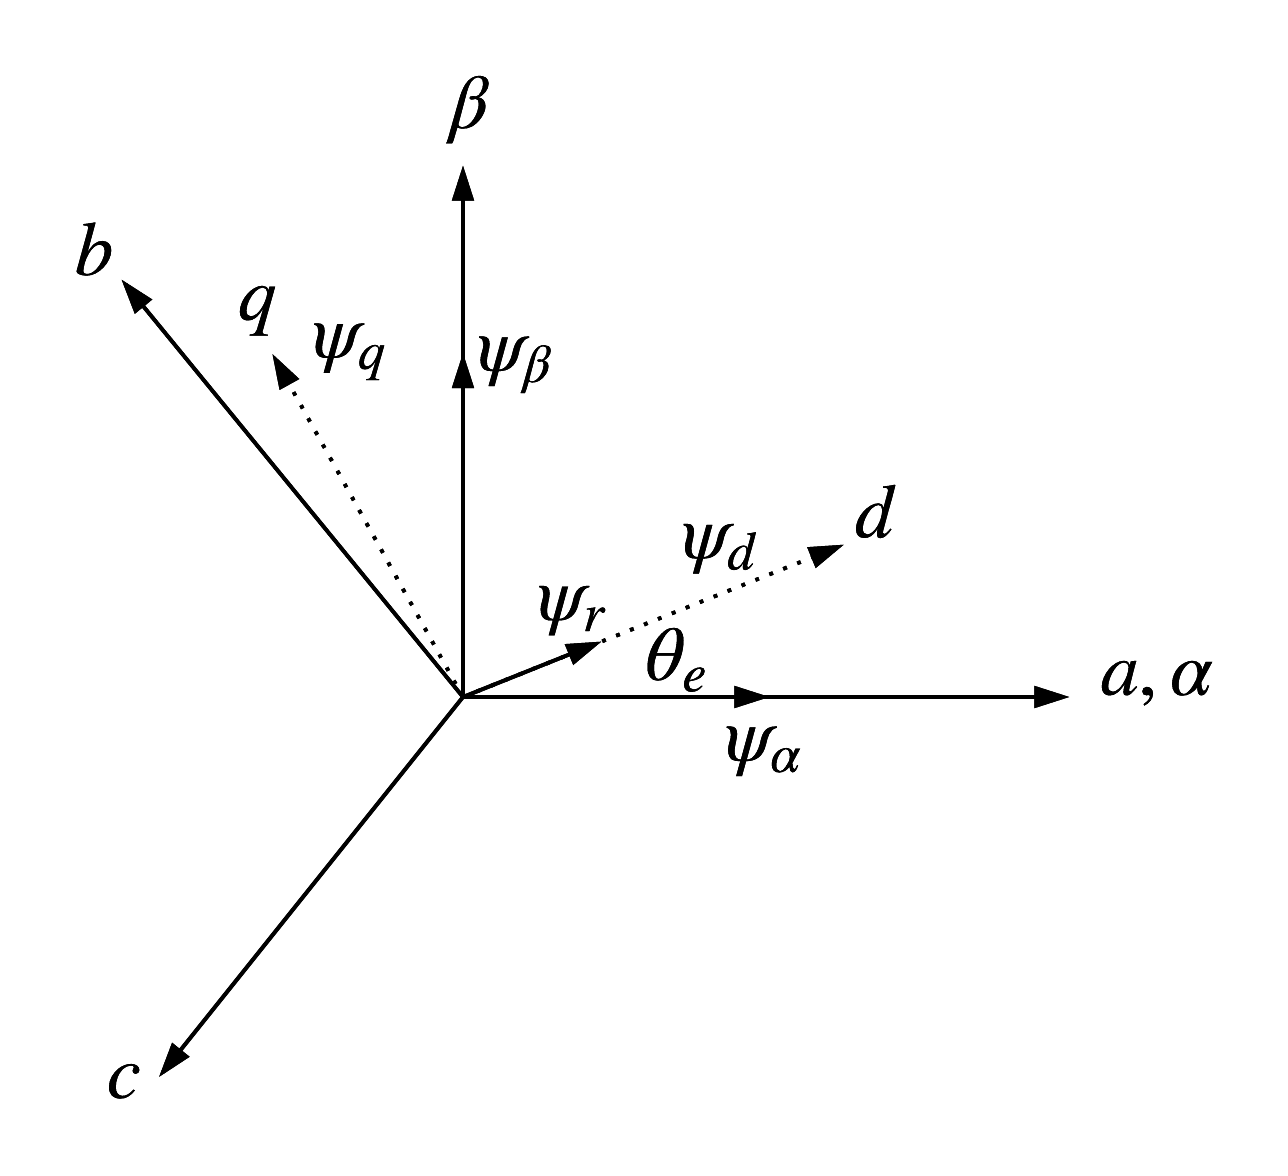
\includegraphics[scale=0.65]{chapter0/phasordig}
\caption{Phasor diagram of the field oriented drive system}
\label{phasor}
\end{figure}

and it is quite significant to synthesize the concept of field-oriented control. In this model it can be seen from the torque expression (2.5) that, if the flux along the q-axis
can be made zero then all the flux is aligned along the d-axis and, therefore, the torque can be instantaneously controlled by controlling the current along q-axis. Then the question will be how it can be guaranteed that all the flux is aligned along the d-axis of the machine. When three-phase voltages are applied to the machine, they produce three-phase fluxes both in the stator and the rotor. The three phase fluxes can be represented in a two phase stationary ($\alpha$-$\beta$) frame. If these two phase fluxes along ($\alpha$-$\beta$) axes are represented by a single-vector then all the machine flux will be aligned along that vector. This vector is commonly specified as d-axis which makes an angle $\theta_{e}$ with the stationary frame $\alpha$-axis, as shown in \autoref{phasor}. The q-axis is set perpendicular to the d-axis. The flux along the q-axis in this case will be obviously zero. The phasor diagram \autoref{phasor} presents these axes. When the machine input currents change sinusoidally in time, the angle $\theta_{e}$ keeps changing. Thus the problem is to know the angle $\theta_{e}$ accurately, so that the d-axis of the d-q frame is locked with the flux vector.\\


The control inputs can be specified in two phase synchronously rotating d-q frame as $i_{ds}^{\omega}$ and $i_{qs}^{\omega}$ such that $i_{ds}^{\omega}$ being aligned with the d-axis or the flux vector. These two phase synchronous control inputs are converted into two phase stationary quantities and then to three phase stationary control inputs. To accomplish this the flux angle $\theta_{e}$ must be known precisely. The angle $\theta_{e}$ can be found either by Direct Field Orientation control (DFO) or by Indirect Field Orientation control (IFO). The controller implemented in this fashion that can achieve a decoupled control of the flux and the torque is known as field oriented controller. The block diagram is shown in the \autoref{foc} In the field-oriented controller the flux can be regulated in the stator, air-gap or rotor flux orientation \cite{Vas}-\cite{Lipo}.


\begin{figure}[h]
\centering
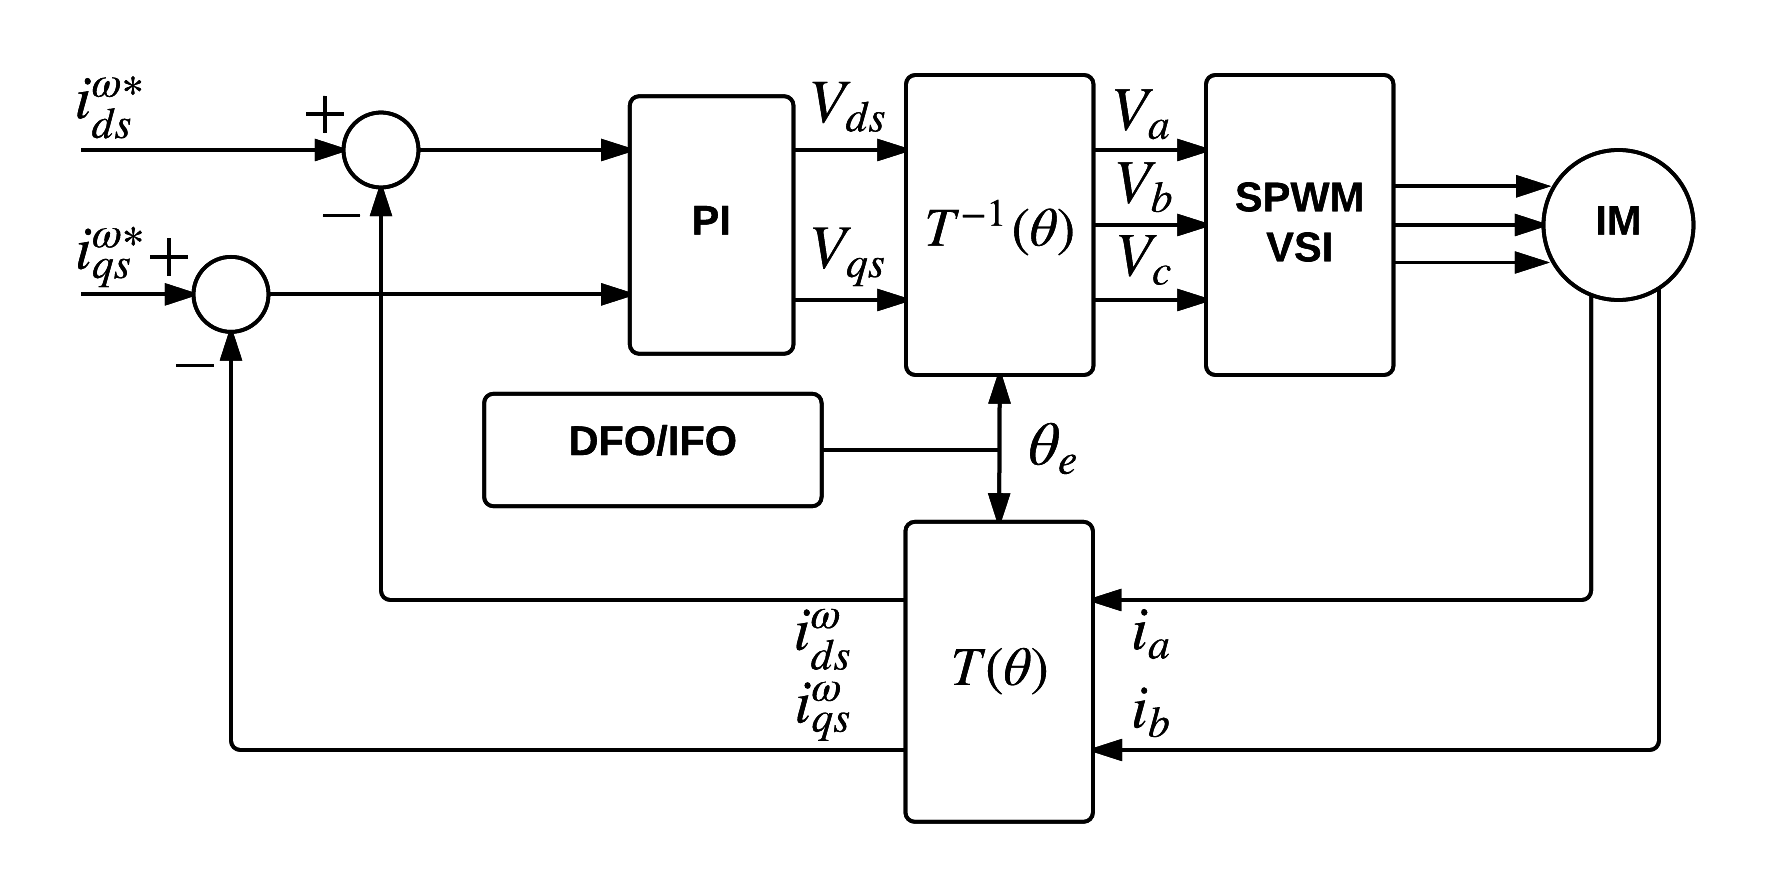
\includegraphics[scale=0.73]{chapter0/foc}
\caption{Field oriented induction motor drive system}
\label{foc}
\end{figure}

The control algorithm for calculation of the rotor flux angle $\theta_{e}$ using IFO control is shown in the \autoref{ifoc}. This algorithm is based on the assumption that, the flux along the q-axis is zero, which forces the command slip velocity to be $\omega_{sl}=i_{qs}^{\omega}/(\tau_{r}i_{ds}^{\omega})$ as a necessary and sufficient condition to guarantee that all the flux is aligned with d-axis and the flux along q-axis is zero. The angle $\theta_{e}$ can then be determined as the sum of the slip and the rotor angles after integrating the respective velocities. This slip angle includes the necessary and sufficient condition for decoupled control of flux and torque. The rotor speed can be measured directly by using an encoder or can be estimated. In case the rotor speed is estimated, the control technique is known as sensorless control. This concept will be studied in detail in the following chapters. \autoref{dfo} shows the control algorithm block diagram for DFO control. In this technique the flux angle $\theta_{e}$ is classically calculated by sensing the air-gap flux through the use of flux sensing coils, or can be calculated by estimating the flux along the d-q axes using the voltage and current signals.

\begin{figure}[h]
\centering
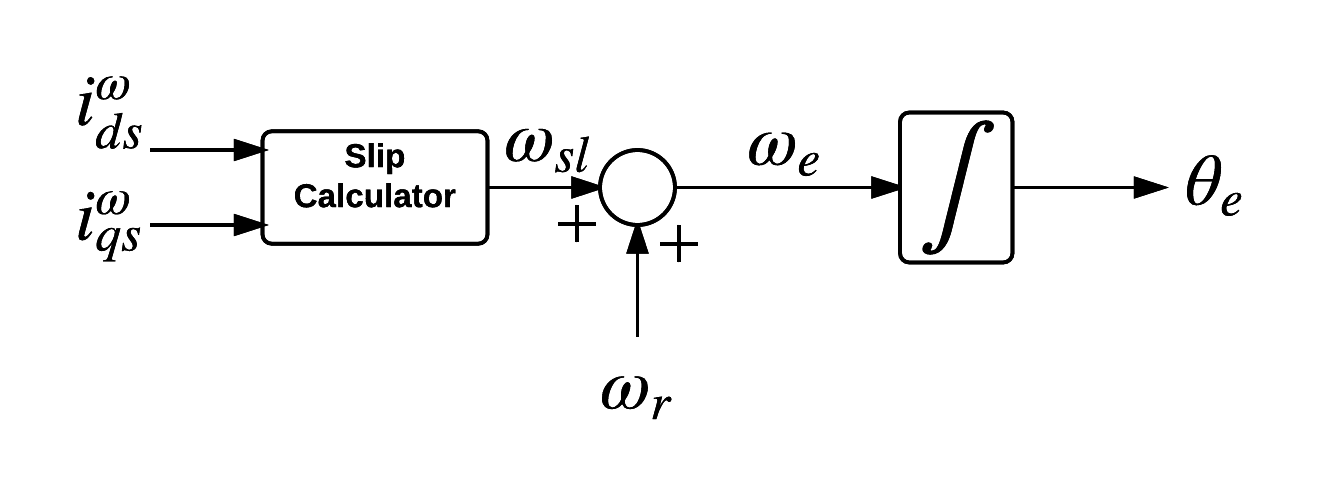
\includegraphics[scale=0.85]{chapter0/ifoc}
\caption{Indirect field oriented drive system}
\label{ifoc}
\end{figure}

\begin{figure}[h]
\centering
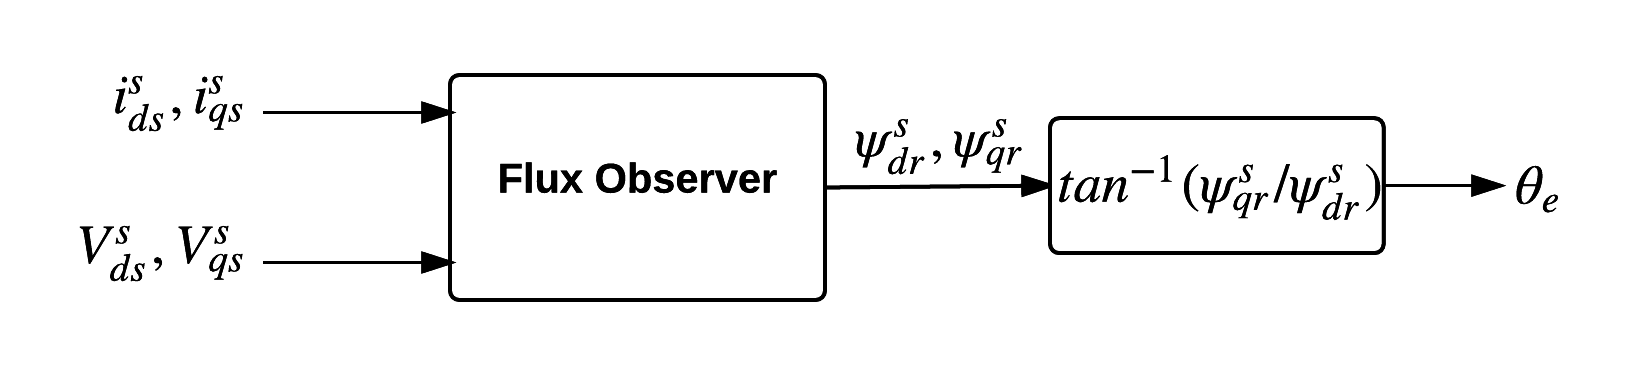
\includegraphics[scale=0.8]{chapter0/dfo}
\caption{Direct field oriented drive system}
\label{dfo}
\end{figure}

\subsection{Direct field orientation (DFO)}

The DFO control and sensorless control rely heavily on accurate flux estimation. DFOC is most often used for sensorless control, because the flux observer used to estimate the synchronous speed or angle can also be used to estimate the machine speed. Investigation of ways to estimate the flux and speed of the induction machine has also been extensively studied in the past two decades. Classically, the rotor flux was measured by using a special sensing element, such as Hall effect sensors placed in the air-gap. An advantage of this method is that additional required parameters, $L_{lr}$, $L_{m}$, and $L_{r}$ are not significantly affected by changes in temperature and flux level. However, the disadvantage of this method is that a flux sensor is expensive and needs special installation and maintenance. Another flux and speed estimation technique is saliency based with fundamental or high frequency signal injection. One advantage of saliency technique is that the saliency is not sensitive to actual motor parameters, but this method fails at low and zero speed level. When applied with high frequency signal injection \cite{jansen}, the method may cause torque ripples, and mechanical problems.\\

Gabriel \cite{Gabrie} avoided the special flux sensors and coils by estimating the rotor flux from the terminal quantities (stator voltages and currents). This technique requires the knowledge of the stator resistance along with the stator, rotor leakage inductances and magnetizing inductance. This method is commonly known as the Voltage Model Flux Observer (VMFO). The stator flux in the stationary frame estimated by the equations:


\begin{align}
\psi_{ds}^s&=V_{ds}^s-R_{s}i_{ds}^s\\
\psi_{qs}^s&=V_{qs}^s-R_{s}i_{qs}^s
\end{align}
Then the rotor flux can be expressed as:
\begin{align}
\psi_{dr}^s&=\frac{L_{r}}{L_{m}}(\psi_{ds}^s-\sigma i_{ds}^s)\\
\psi_{qr}^s&=\frac{L_{r}}{L_{m}}(\psi_{qs}^s-\sigma i_{qs}^s)
\end{align}

In this model, integration of the low frequency signals, dominance of stator resistance voltage drop at low speed and leakage inductance variation result in a less precise flux estimation. Integration at low frequency is studied by \cite{jun} and three different alternatives are given. Estimation of rotor flux from the terminal quantities depends on parameters such as stator resistance and leakage inductance. The study of parameter sensitivity shows that the leakage inductance can significantly affect the system performance such as stability, dynamic response, and utilizations of the machine and the inverter.\\


The Current Model Flux Observer (CMFO) is an alternative approach to overcome the problems of leakage inductance and stator resistance at low speed. In this model flux can be estimated as:
\begin{align}
\psi_{dr}^s=-\frac{1}{\tau_{r}}\psi_{dr}^s-\omega_{r}\psi_{qr}^s+\frac{L_{m}}{\tau_{r}}i_{ds}^s\\
\psi_{qr}^s=-\frac{1}{\tau_{r}}\psi_{qr}^s-\omega_{r}\psi_{dr}^s+\frac{L_{m}}{\tau_{r}}i_{qs}^s
\end{align}

However, it does not work well at high speed due to its sensitivity to the rotor resistance. Jansen \cite{pl} did an extensive study on VMFO and CMFO based direct field orientation control, discussed the design and accuracy assessment of various flux observers, compared them, and analyzed the alternative flux observers. To further improve the observer performance, closed-loop rotor flux observers are proposed which use the estimated stator current error \cite{pl,gc} or the estimated stator voltage error \cite{gc} to estimate the rotor flux. Furthermore, Lennart \cite{len} proposed reduced order observers for this task.

\subsection{Indirect field orientation control (IFOC)}


In indirect field orientation, the synchronous speed $\omega_{e}$ is the same as the instantaneous speed of the rotor flux vector $\psi_{dr}^{\omega}$ and the d-axis of the d-q coordinate system is exactly locked on the rotor flux vector (rotor flux vector orientation). This facilities the flux control through the magnetizing current $i_{ds}^{\omega}$ by aligning all the flux with the d-axis while aligning the torque producing component of the current with the q-axis. After decoupling the rotor flux and torque producing component of the current components, the torque can be instantaneously controlled by controlling the current $i_{qs}^{\omega}$. The requirement to align the rotor flux with the d-axis of the d-q coordinate system means that the flux along the q-axis must be zero. This means that the current through the q-axis of the mutual inductance is zero.\\

Based on this restriction $\omega_{sl}$ is :

\begin{align}
\omega_{sl}=\frac{i_{qs}^{\omega}}{(\tau_{r}i_{ds}^{\omega})}
\end{align}

These relations suggest that flux and torque can be controlled independently by specifying d-q axis currents provided the slip frequency is satisfied (2.12) at all instants.\\


The concept of indirect field oriented control developed in the past has been widely studied by researchers during the last two decades. The rotor flux orientation is both the original and usual choice for the indirect orientation control. Also the IFO control can be implemented in the stator and air-gap flux orientation as well. De Doncker \cite{doncker} introduced this concept in his universal field oriented controller. In the air-gap flux the slip and flux relations are coupled equations and the d-axis current does not independently control the flux as it does in the rotor flux orientation. For the constant air-gap flux orientation, the maximum of the produced torque is \%20 less than that of the other two methods \cite{sul}. In the stator flux orientation, the transient reactance is a coupling factor and it varies with the operating conditions of the machine. In addition, Mircea \cite{mirc} shows that among these methods, rotor flux oriented control has linear torque curve. Therefore, the most commonly used choice for IFO is the rotor flux orientation.\\

The IFOC is an open loop, feed forward control in which the slip frequency is fed forward guaranteeing the field orientation. This feed forward control is very sensitive to the rotor open circuit time constant $\tau_{r}$. Therefore, $\tau_{r}$ must be known in order to achieve a decoupled control of torque and flux components by controlling $i_{ds}^{\omega}$ and $i_{qs}^{\omega}$ , respectively. When $\tau_{r}$ is not set correctly, the machine is said to be detuned and the performance will become sluggish due to loss of decoupled control of torque and flux. The measurement of the rotor time constant, its effects on the system performance and its adaptive tuning to the variations resulting during the operation of the machine have been studied extensively in the literature \cite{rl}-\cite{krisn}. Lorenz, Krishnan and Novotny \cite{rl}-\cite{krisn} studied the effect of temperature and saturation level on the rotor time constant and concluded that it can reduce the torque capability of the machine and torque/amps of the machine. The detuning effect becomes more severe in the field-weakening region. Also, it results in a steady-state error and, transient oscillations in the rotor flux and torque. Some of the advanced control techniques such as estimation theory tools and adaptive control tools are also studied to estimate rotor time constant and other motor parameters \cite{ca}-\cite{jm}.\\


\section{Variable speed control using advance control algorithms}

There are two issues in motion control using field oriented controlled (FOC) induction machine drives. One is to make the resulting drive system and the controller robust against parameter deviations and disturbances. The other is to make the system intelligent to adjust the control system itself to environment changes and task requirements. If the speed regulation loop fails to produce the command current correctly, than the desired torque response will not be produced by the induction machine. In addition, such a failure may cause the degradation of slip command. As a result, a satisfactory speed regulation is extremely important not only to produce desired torque performance from the induction machine but also to guarantee the decoupling between control of torque and flux.\\

Conventionally, a PI controller has been used for the speed regulation to generate a command current for last two decades, and accepted by industry because of its simplicity. Even though, a well tuned PI controller performs satisfactorily for a field oriented induction machine during steady state. The speed response of the machine at transient, especially for the variable speed tracking, may sometimes be problematic. In last two decades, alternative control algorithms for the speed regulation were investigated. Among these, fuzzy logic, sliding mode, and adaptive nonlinear control algorithms gained much attention.\\

A traditional rotor flux oriented induction machine drive offers a better control performance but it often requires additional sensors on the machine. This adds to the cost and complexity of the drive system. To avoid these sensors on the machine, many different algorithms are proposed for the last three decades to estimate the rotor flux vector and rotor shaft speed. The recent trend in field oriented control is to use such algorithms based on the terminal quantities of the machine for the estimation of the fluxes and speed. They can easily be applied to any induction machine. Therefore, our focus in this study is also on these algorithms.\\


Before looking into individual approaches, the common problems of the speed and flux estimation are discussed briefly for general field orientation and state estimation algorithms.
 \begin{itemize}
 \item{\textbf{Parameter sensitivity:} One of the important problems of the sensorless control algorithms for the field oriented induction machine drives is the insufficient information about the machine parameters which yield the estimation of some machine parameters along with the sensorless structure. Among these parameters stator resistance, rotor resistance and rotor time constant play more important role than the other parameters since these values are more sensitive to temperature changes. The knowledge of the correct stator resistance $R_{s}$ is important to widen the
operation region toward the lower speed range. Since at low speeds the induced voltage is low and stator resistance voltage drop becomes dominant, a mismatching stator resistance induces instability in the system. On the other hand, errors made in determining the actual value of the rotor resistance $R_{r}$, may cause both instability of the system and speed estimation error proportional to $R_{r}$ \cite{gy}. Also, correct $\tau_{r}$ value is vital decoupling factor in IFOC}
 
\item{\textbf{Pure Integration:} The other important issue regarding many of the topologies is the integration process inherited from the induction machine dynamics where an integration process is needed to calculate the state variables of the system. However, it is difficult both to decide on the initial value, and prevent the drift of the output of a pure integrator. Usually, to overcome this problem a low-pass filter replaces the integrator.}

\item{\textbf{Overlapping loop Problems:} In a sensorless control system, the control loop and the speed estimation loop may overlap and these loops influence each other. As a result, outputs of both of these loops may not be designed independently,  in some bad cases this dependency may influence the stability or performance of the overall system.}
\end{itemize}
\vspace{1cm}
The algorithms, where terminal quantities of the machine are used to estimate the fluxes and speed of the machine are categorized in two basic groups. First one is ``the open loop observers," in a sense that the on-line model of the machine does not use the feedback correction. Second one is ``the closed loop observers" where the feedback correction is used along with the machine model itself to improve the estimation accuracy. These two basic groups can also be divided further into subgroups based on the control method used. These can be summarized as:\\

Open loop observers based on:\\
- Current model\\
- Voltage model\\
- Full-order observer\\


Closed loop observers based on:\\
- Model Reference Adaptive Systems (MRAS)\\
- Kalman filter techniques\\
- Adaptive observers based on both voltage and current model\\
- Neural network flux and speed estimators\\
- Sliding mode flux and speed estimators\\

Current model based open loop observers use the measured stator currents and rotor velocity. The velocity dependency of the current model is very important since this means that although using the estimated flux eliminates the flux sensor, the position sensor is still required. On the other hand, voltage model based open loop observers \cite{M}-\cite{gc} use the measured stator voltage and current as inputs. A full-order open loop observer can be formed using only the measured stator voltage and rotor velocity as inputs where the stator current appears as an estimated quantity. Because of its dependency on the stator current estimation, the full order observer will not exhibit better performance than the current model. Furthermore, parameter sensitivity and observer gain are the problems to be tuned in a full order observer design \cite{br}. These open-loop observer structures are all based on the induction machine model, and they do not employ any feedback. Therefore, they are quite sensitive to parameter variations, which yield the estimation of some machine parameters along with the sensorless structure.\\
\vspace{1cm}\\

To produce more robust structures to parameter variations some kind of feedback may be helpful. For this purpose many closed loop topologies are proposed using different induction machine models and control methods. Among these MRAS attracts attention and several different algorithms are produced. In MRAS a comparison is made between the outputs of two estimators. The estimator which does not contain the quantity to be estimated can be considered as a reference model of the induction machine. The error between these two estimators is used as an input to an adaptation mechanism. The estimated rotor speed in the adjustable model is changed in such a way that the difference between two estimators converges to zero asymptotically, and the estimated rotor speed will be equal to actual rotor speed. The basics of the analysis and design of MRAS are discussed in \cite{Vas, booksul}. In \cite{gy, J}. In \cite{cs} similar speed estimators are proposed based on the MRAS, and a secondary variable is introduced as the reference quantity by letting the rotor flux through a first-order delay instead of a pure integration to nullify the offset. However, their algorithms produce inaccurate estimated speed if the excitation frequency goes below certain level. In addition these algorithms suffer from the machine parameter uncertainties since the parameter variation in the reference model cannot be corrected. Zhen \cite{lz} proposed an interesting MRAS structure that is built with two mutual MRAS schemes. In this structure, the reference model and the adjustable models are interchangeable. For rotor speed estimation, one model is used as reference model and other model is used as adjustable model. The pure integration is removed from reference model. \cite{me} supported the MRAS scheme with ANN using its training and modeling of non-linear systems. MRAS scheme is also used for the on-line adaptation of the motor parameters in field oriented control techniques \cite{ca, kubota}.\\

Kalman filter (KF) is another method employed to identify the speed and rotor flux of an induction machine based on the measured quantities such as stator current and voltage \cite{kim}. Kalman filter approach is based on the system model and a mathematical model describing the induction motor dynamics for the use of Kalman filter application. Parameter deviations and measurement disturbance are taken into consideration in KF covariance matrices of the KF must be properly initialized. KF works for linear systems and for non linear induction motor model extended Kalman filter (EKF) is used. However, KF approach is computationally intensive and depends on the accuracy of the model of the motor. In the EKF model proposed by  one can estimate rotor fluxes and rotor speed which makes the field orientation. EKF is also used for online parameter estimation of induction motor \cite{Vas, lcz}. Reduced order models are also proposed to shorten and speed up the complex EKF algorithm \cite{ekf}. A new KF technique for non-linear systems, Unscented Kalman Filter (UKF), is applied to induction machine state estimatio, which is a derivative free KF technique which avoids costly calculation of Jacobian matrix, linearization of the estimates \cite{ukf}.\\


Another method used for the sensorless control of induction motor is the neural network technique, which is based on a learning process. It has the advantage of tolerating machine parameter uncertainties. For speed estimation, a two-layered neural network, based on back propagation technique, is used and the neural network outputs are compared with the actual measurement values and error then back- propagated to adjust the weights such that the estimated speed converges to actual one. The neural network based sensorless control algorithms have the advantages of fault-tolerant characteristics. However, because of the neural network learning process these algorithms may suffer from the computational intensity.\\

Another approach is sliding mode control for FOC of induction machine. In the sliding mode technique, the control action is very strong and being switched into either ``on" or ``off" at high frequency. The command signals control directly the power devices. This type of control is also favorable because ``on-off" is the only admissible mode of operation for the power converters. Therefore, it seems more natural to employ the algorithm towards discontinuous control.\\

In addition to the algorithms mentioned above, some of the proposed work is hard to classify because of their combined structure. In \cite{J}, a nonlinear high- gain observer structure is proposed, and it is claimed that with the exact knowledge of stator resistance, flux and speed estimation convergence is guaranteed.

\section{Conclusion}

The literature review of DFOC, IFOC, flux, position and speed estimation and speed control can be summarized as:
\begin{itemize}

\item{The DFOC and IFOC are the methods for instantaneous torque and speed control of an induction motor drive system. These methods can be implemented with or without a speed sensor. An IFOC is synthesized by properly controlled slip frequency which is necessary for the field-orientation}\\
\item{The main problem of an IFO drive system is the rotor time constant deviation. The drive system torque control performance decreases if the rotor time constant is not set precisely. Therefore, on-line estimation is necessary and is one of the main challenges for better performance of an IFOC. Most of the techniques proposed so far either need some special hardware or are very complex with respect to the software and require intensive calculations which put extra burden on the processor.}\\
%\item{The main problem in DFO control is precise rotor flux or position observation. This observation from terminal quantities is more desirable than the one including additional hardware.}\\
\item{Voltage model and current model flux observers are the two most common ways to estimate the flux using the terminal quantities. The voltage model flux observer is dominated by stator IR drop at low speed, whereas the current model flux observer has problems of rotor time constant variations. Also the current model flux observer requires the rotor speed. Therefore, if the flux observer is being used for the sensorless control, an error in the estimated speed will be fed back in to the system. Thus will affect the observer accuracy.}\\
\item{The proposed open-loop observers can be simple in the structure but they are susceptible to variety of errors that become specially detrimental at low stator frequencies, including measurement, noise digital approximation errors, parameter detuning and DC offset in measurements, which ultimately may drive the observer instability.}\\
\item{For the time varying system model problems, closed-loop observers are proposed here feedback correction is used along with the machine model itself to improve the estimation accuracy. The algorithmic complexity and calculation intensity looks higher when compared with former solutions but the recent processors are fast enough to solve these algorithms in real-time applications. They also require a strong mathematical background to deal with.}
\end{itemize}


\chapter{Modeling influence on a Social Network using Interaction Characteristics}


\section{Introduction}
% no \IEEEPARstart
The importance of social networks has been realized since the advent of Facebook in 2004 as well as other social networks such as Twitter, Flickr and Instagram. When a user posts a message on social media, other users in the network respond to the content by performing certain actions which create cascading effects within the network and is visible in the form of further activity. The fact that a message from one user prompted certain reactions from other users is an indication of the influence of one user over others in the network. This can be used to enhance the visibility of a product, viral marketing, and spreading awareness or even during disasters to alert citizens, or spreading hatred or rumors. \\

It is due to this popularity social media analytics has attracted a lot of attention from the research communities in machine learning \cite{aps:1} \cite{aps:8} \cite{aps:4}, preference learning \cite{aps:9}, recommendation systems, data mining \cite{aps:10}, information retrieval \cite{aps:11} etc. Social networks belong to the category of networks called strategic network models where the relation between nodes is determined by the choice of the members involved, not by a random rule. This means that the characteristics of nodes are important in determining whether links shall be formed. This also decides whether the information that is diffused can reach more nodes of the network. Chen \textit{et. al} and Subbian \textit{et. al} have proposed methods for finding influential nodes which use the process of information diffusion or social capital to discover the nodes with high diffusion centrality \cite{aps:12} \cite{aps:13}. Holander \textit{et. al} have argued that use of Eigenvector centrality as a measure is insufficient in deciding the and ranking influential nodes in online networks \cite{aps:15} \cite{aps:14}. \\

Influence maximization problem is a NP hard problem of identifying the subset of nodes in a social network that would maximize the coverage of information in the graph through diffusion. However the problem of assigning influence scores to every node in the graph is different compared to Influence Maximization since the former is a measurement problem, while the latter is a subset selection problem and both have different objectives \cite{aps:12} \cite{aps:13}. In influence ranking, Klout rank proposed by Rao \textit{et al}. has achieved significant breakthrough in calculating the current influence or rank of the user in the social network by analyzing the interaction characteristics generated by the user on a social network in the preceding 90 days \cite{aps:14}. The mathematical model implemented to calculate the Klout rank uses a feature vector of 3600 attributes.  The parameters of the model have been tuned by analyzing 45 billion interactions of various users collected from online networks. Machine learning techniques applied on data to create a predictive model has been investigated by Alexy \textit{et al}. \cite{aps:19} \cite{aps:17}. The model uses interaction characteristics such as number of mentions over time to create a PageRank like score for ranking users by their influence. Behnam \textit{et al}. \cite{aps:18} modeled influence using metrics such as number of followers and their ratio of affection to a particular topic. However previous literature ignored making up decision rules and understanding complex relationships between features that could lead to development of an objective criteria for calculating and comparing influence.\\


In this paper, attributes that are accumulated by the behavior of a person on the social network are used. The key assumption is that these attributes have a relationship with the influence of the person and can be used to create a feature vector to model the influence. The online characteristics that can be measured by information extracted from an online social network are impressions, clicks, likes, comments, re-shares, followers. Such attributes are difficult to emulate or artificially enhance and hence are appropriate indicators for developing an objective criteria for assessing the influence.\\

We have conducted experiments on the real world dataset from twitter to validate the effectiveness of the proposed approach. \\

The highlights of the paper are summarized as follows :\\

\begin{enumerate}
  \item A machine learning approach to study the comparison of influencers in the social network using various algorithms and their effectiveness on the data.
  \item Analysis of various features and their use in training and building a model.
        \item Use of feature selection, feature ranking techniques and their effect on the model and the predictions. Thus obtaining a smaller set of predictors that decide influence within a network.
        \item Validation of the model and comparisons to establish which of the techniques has best results. 
        \\
\end{enumerate}
	

Section II presents the related work in the field and the introduction to machine learning models and other techniques implemented in the paper. Section III formulates the problem, provides the objective function and then proposed approach. Section IV provides information about the data set, the methodology, experimental design and results. The conclusion is given in Section V.

\section{Related Work}

\subsection{Twitterrank: finding topic-sensitive influential twitterers}
The TwitterRank algorithm was implemented for studying people who are the most influential in the social network. The algorithm is based on the hypothesis that the measure of influence of a person is related to both the topical similarity between twitterers and the link structure. The authors argue that they could find evidence to support the theory which states that more followers a person has in a social network the more is the influence i.e. in-degree of a node is proportional to its influence in the network. The algorithm works on the assumption that there exists homophily within twitter i.e. same interests decide the relationship between the users. However no correlation is presented in the form of a degree distribution to prove existence of homophily \cite{aps:20} \cite{aps:16}. 


\subsection{Finding influencers using social capital}
The concept of “social capital” is proposed by the authors. According to them "Social capital" is computed by means of bonding and bridging capital. The bonding capital is defined as the ability to calibrate similar people against each other. The bridging capital is defined as the ability to connect diverse people. A bridging node is like an interdisciplinary researcher who connects different communities of researchers and a bonding node is a good researcher in a domain. It is argued that such nodes create a value throughout the network and this value is shared by them. The hypothesis is that this value is proportional to the influence of the node amongst other nodes it is connected to in the network. The social capital and its distribution amongst the nodes is based on the concept of distance based utility which is seen in strategic network formation process. The distance-based utility concept assumes that all players (nodes) have a utility in the network that is alike. Furthermore it takes into account only the benefits that a node in the network derives from other nodes to which it has indirect links. For the purpose of computing the value derived through the indirect links only links having minimum path length from source to destination are considered. These two features are considered as drawbacks of the distance-based utility in general and the same have been seen in the social capital based approach \cite{aps:13}.

\subsection{Geo-social Influence Spanning Maximization}
The Influence maximization problem has been modified to include the physical location of the social users in an attempt to solve the NP- Hard problem of identifying a small set of users that can influence the maximum number of users in a network. The technique measures influence as a factor of diffusion potential of a node. It is computationally expensive and may yield results that cannot guarantee global optimal solution due to the vast search space. The technique proposed uses greedy algorithm to identify the top "k" seeds that can propagate the influence across the network. The technique also proposes a hybrid indexing structure OIR*- tree which combines the features of an ordered influential user list and R*-tree. The indexing structure doesn’t consider the changing in the influence with time. The space complexity of this approach is higher as the influential nodes have to be stored. This approach is not useful for measuring influence of the node in a network \cite{aps:21}.

\subsection{Mining Time-Dependent Influential Users in Facebook Fans Group}
"Klout rank" is a popular method of using machine learning techniques to calculate the influence of a user in a network. The klout score is computed based on the statistics calculated about the user from various social platforms and a score is assigned to them. The technique however doesn’t consider that influence is time dependent. This means that a user may not have a high average klout score but could be influential at a particular time period. Klout also works on a “black box” model that doesn’t explain what can affect the influence of users in a network. Bias/variance graphs are not presented to indicate whether having 3600 features can lead to overfitting \cite{aps:23} \cite{aps:22}.


% An example of a floating figure using the graphicx package.
% Note that \label must occur AFTER (or within) \caption.
% For figures, \caption should occur after the \includegraphics.
% Note that IEEEtran v1.7 and later has special internal code that
% is designed to preserve the operation of \label within \caption
% even when the captionsoff option is in effect. However, because
% of issues like this, it may be the safest practice to put all your
% \label just after \caption rather than within \caption{}.
%
% Reminder: the "draftcls" or "draftclsnofoot", not "draft", class
% option should be used if it is desired that the figures are to be
% displayed while in draft mode.
%
%\begin{figure}[!t]
%\centering
%\includegraphics[width=2.5in]{myfigure}
% where an .eps filename suffix will be assumed under latex, 
% and a .pdf suffix will be assumed for pdflatex; or what has been declared
% via \DeclareGraphicsExtensions.
%\caption{Simulation results for the network.}
%\label{fig_sim}
%\end{figure}

% Note that the IEEE typically puts floats only at the top, even when this
% results in a large percentage of a column being occupied by floats.


% An example of a double column floating figure using two subfigures.
% (The subfig.sty package must be loaded for this to work.)
% The subfigure \label commands are set within each subfloat command,
% and the \label for the overall figure must come after \caption.
% \hfil is used as a separator to get equal spacing.
% Watch out that the combined width of all the subfigures on a 
% line do not exceed the text width or a line break will occur.
%
%\begin{figure*}[!t]
%\centering
%\subfloat[Case I]{\includegraphics[width=2.5in]{box}%
%\label{fig_first_case}}
%\hfil
%\subfloat[Case II]{\includegraphics[width=2.5in]{box}%
%\label{fig_second_case}}
%\caption{Simulation results for the network.}
%\label{fig_sim}
%\end{figure*}
%
% Note that often IEEE papers with subfigures do not employ subfigure
% captions (using the optional argument to \subfloat[]), but instead will
% reference/describe all of them (a), (b), etc., within the main caption.
% Be aware that for subfig.sty to generate the (a), (b), etc., subfigure
% labels, the optional argument to \subfloat must be present. If a
% subcaption is not desired, just leave its contents blank,
% e.g., \subfloat[].


% An example of a floating table. Note that, for IEEE style tables, the
% \caption command should come BEFORE the table and, given that table
% captions serve much like titles, are usually capitalized except for words
% such as a, an, and, as, at, but, by, for, in, nor, of, on, or, the, to
% and up, which are usually not capitalized unless they are the first or
% last word of the caption. Table text will default to \footnotesize as
% the IEEE normally uses this smaller font for tables.
% The \label must come after \caption as always.
%
%\begin{table}[!t]
%% increase table row spacing, adjust to taste
%\renewcommand{\arraystretch}{1.3}
% if using array.sty, it might be a good idea to tweak the value of
% \extrarowheight as needed to properly center the text within the cells
%\caption{An Example of a Table}
%\label{table_example}
%\centering
%% Some packages, such as MDW tools, offer better commands for making tables
%% than the plain LaTeX2e tabular which is used here.
%\begin{tabular}{|c||c|}
%\hline
%One & Two\\
%\hline
%Three & Four\\
%\hline
%\end{tabular}
%\end{table}


% Note that the IEEE does not put floats in the very first column
% - or typically anywhere on the first page for that matter. Also,
% in-text middle ("here") positioning is typically not used, but it
% is allowed and encouraged for Computer Society conferences (but
% not Computer Society journals). Most IEEE journals/conferences use
% top floats exclusively. 
% Note that, LaTeX2e, unlike IEEE journals/conferences, places
% footnotes above bottom floats. This can be corrected via the
% \fnbelowfloat command of the stfloats package.

\section{Mathematical Model}
An online social network is represented as a graph G = (V, E) with nodes (V) represents the number of users and edges (E) denote friendship between two users. In most of the social networks the users send requests to other users to form a relationship. The acceptance of this request is then a undirected link. Usually the friendhsip links in a social networking graph can be both undirected (Facebook) as well as directed (Twitter). The nodes also have properties that are due to the membership of this network. These properties are derived from membership of the network and are varied by the influence of his behavior on the network and the networks influence on his behavior i.e. co-evolution.  \\

The measurement problem of calculating the influence shall become a problem of supervised learning. Supervised learning algorithms are of many types and there is no single algorithm that can work on any given supervised learning problems. Neural networks perform well if the task involves identifying complex set of dependencies and identifying these dependencies. However the best configuration of a neural network has to be determined experimentally.\\


\subsection{Calculation of Influence Score}
A feature vector $x_i$ is constructed for each user from the set of features extracted for each user from Twitter as shown in Table 1. Then a Given a set of N training examples of the form {($x_1$, $y_1$), …, ($x_n$, $y_n$)} such that $x_i$ is the feature vector of the $i^{th}$ example and $y_i$ is its class label. The algorithm creates a function $g: X \rightarrow Y$ where X is the input space and Y is the output space.

\begin{table}[!h]
\renewcommand{\arraystretch}{1.3}
\caption{Feature vector}
\label{table}
\centering
\begin{tabular}{|c|c|c|c|}
  \hline
\multicolumn{1}{|c|}{\textbf{Sr. No}} & \multicolumn{1}{c|}{\textbf{Feature list}} & \multicolumn{1}{c|}{\textbf{Sr. No}} & \multicolumn{1}{c|}{\textbf{Feature list}}\\
  \hline
  1 & Follower count & 5 & Following count\\
  \hline
  2 & Listed count & 6 & mentions received\\
  \hline
  3 & retweets received & 7 & mentions received\\
  \hline
  4 &  retweets sent & 8 & posts\\
  \hline
\end{tabular}
\end{table}

\subsection{Model Representation}

\subsubsection{Artificial Neural Networks}
Artificial neural networks are composed of input layers, hidden layers and output layers. The number of hidden layers ideally should be more as they can compute more nonlinear relationships between the inputs. However, it is important to avoid over-fitting while deciding the number of hidden layers and the number of hidden units. The input feature matrix $X$ and the weight matrix of the $W_{21}$ $(\theta_{1})$ and the result are given to the sigmoid function to decide which neurons of the hidden layer 1 i.e. ($a_{1}$) are activated. The output of this hidden layer is the multiplied with the second weight matrix $W_{31}$ $(\theta_{2})$ and so on till the output layer. The back-propagation algorithm is then used to obtain the adjusted weights. The cost function of the network for the classification problem is provided in Eqn. (1) and the penalty term (regularization) is used to it for preventing over-fitting is provided in Eqn.(2).\\


\begin{figure}
\centering
\fbox{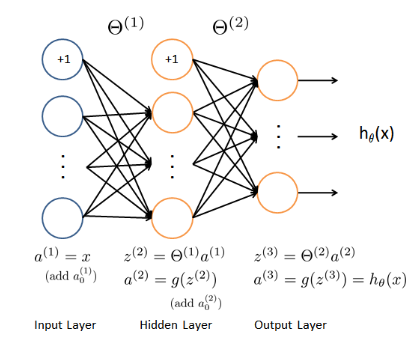
\includegraphics[scale=0.45]{fignn.png}}
\caption{Neural Network Architecture with Backpropagation}
\label{fig 1}
\end{figure}



\subsubsection{Cost Function - Artificial Neural Networks}

The cost function is that of the standard regularized logistic regression which is generalized for $k$ outputs instead of one output. For our problem the output is a single value of 0/1 depending upon whose influence in a network is more. The cost function shall be minimized using the back propagation algorithm to get the ideal value of the weights.

\begin{equation}
J(\Theta ) = \frac{a}{b} \sum_{i=1}^{k}\sum_{k=1}^{k} * [-y_{k}^{i}*log((h_{\Theta }(x^{i}))_{k}) - (1-y_{k}^{(i)})*log((h_{\Theta }(x^{i}))_{k})] 
\end{equation}
\begin{equation}
Penalty =  \frac{\lambda }{m}* [\sum_{j=1}^{J1}\sum_{k=1}^{K1}*(\Theta _{(j,k))}^{(1))})^{2} + \sum_{j=1}^{J2}\sum_{k=1}^{K2}*(\Theta _{(j,k))}^{(2))})^{2}]
\end{equation}

\subsubsection{Gradient boosted trees}

Gradient boosting is a technique that combines several weak learners into a strong learner using multiple iterations. Gradient boosting is applied with decision trees of fixed size as the first level learners. The decision tree partitions the input space into disjoint regions and predicts a constant value in each region. The General idea for a gradient boosted tree is to fit a model to the data i.e $F_1$(x) = y . Fit the model to the residuals denoted by $h_{(1)(x)}$ = y - $F_1$(x). Then obtain a new model $F_2$(x) = $F_1$(x) + $h_1$(x). The value of 'm' or the hyper parameter which gives the number of iterations of the residual correction procedure is obtained by cross validation. \\ 





\subsubsection{Gradient Boosted trees}



Model Update rule:

\begin{equation}
F_{m}(x) = F_{(m-1)}(x)) + \sum_{j=1}^{J_m} \gamma_{jm} I (x \epsilon R_{jm}) 
\end{equation}

\subsection{Influence Ranking Algorithm}

The algorithm for comparison of influence between two users whose network features have been collected from Twitter is presented. The parameters of various models are set initially and these values are modified till the ideal values are obtained. The cross validation set is used for this purpose.\\

\begin{algorithm}
\caption{Influencer Ranking model}
\begin{algorithmic}[1]
 \State Set initial seed for random numbers
 \State Set the training control values
 \State Set the tuning grid for parameter search
 \For {each parameter set} do
 \For {each resampling iteration set} do
 \State hold out specific samples
 \State Pre process the data (Center and Scale)
 \State Fit the model on the remaining samples
 \State Predict the held out samples
 
 \EndFor
 \State Calculate the average performance across held out predictions
 \EndFor
 \State Determine the optimal parameter set
 \State Fit the final model to all the training data using optimal parameter set 
 

\end{algorithmic}
\end{algorithm}

\section{Experimental Study}

\subsection{Experiment setting}

The performance of the Influence Ranking algorithm in Section III-(C) is studied to understand the best set of features to measure influence.\\

\subsubsection{Dataset}  
The dataset comprises a standard, pair-wise preference learning task. Each data point describes two individuals whose identities are anonymized and their future references in the paper are made using labels 'A' and 'B'. For each person, 8 pre-computed, non-negative numeric features based on twitter activity are provided. The binary label represents a human judgement about which one of the two individuals is more influential. The Ground truth labels provided are 0/1 to indicate which of the users is more influential. The test set has 5952 entries for which label has to be predicted.

\begin{table}[!h]
\renewcommand{\arraystretch}{1.3}
\caption{Description of the dataset}
\label{table}
\centering
\begin{tabular}{|c|c|c|c|}
  \hline
\multicolumn{1}{|c|}{\textbf{Training set size}} & \multicolumn{1}{c|}{\textbf{Test set size}} & \multicolumn{1}{c|}{\textbf{Feature vector}} & \multicolumn{1}{c|}{\textbf{Classification}}\\
  \hline
  5500 & 5952 &  22 & Binary\\
  \hline
\end{tabular}
\end{table}


\subsection{Results}

The accuracy and performance on test set was measured for the Three layered ANN trained using correlated and uncorrelated predictors.

\begin{table}[H]
\renewcommand{\arraystretch}{1.3}
\caption{Modeling influence using Multilayered Perceptron with Backpropagation}
\label{table}
\centering
\begin{tabular}{|c|c|c|c|}
%\begin{tabular}{|p{0.1in}|p{0.75in}|p{0.51in}|p{.51in}|p{0.51in}|}
  \hline
\multicolumn{1}{|c|}{\textbf{Sample size}} & \multicolumn{1}{c|}{\textbf{Hidden units}} & \multicolumn{1}{c|}{\textbf{Training Accuracy}} & \multicolumn{1}{c|}{\textbf{Training Kappa}}\\
  \hline
  3521 &  16 & 72.29 & 44.55\\
  \hline
  3521 &  24 & 71.29 & 43.42\\
  \hline
  3521 &  32 & 71.55 & 43.04\\
  \hline
\end{tabular}
\end{table}

For above experiment correlated features ($\geq{0.75}$) were removed. Cross validation technique used was X-cross fold with X = 5 and 5 times repeat. Training set accuracy was used as selection criteria for evaluation and hidden units were decided as 16. The trained model gave an accuracy of 0.801 on the test set.


\begin{table}[!h]
\renewcommand{\arraystretch}{1.3}
\caption{Modeling influence using Multilayered Perceptron with Backpropagation}
\label{table}
\centering
\begin{tabular}{|c|c|c|c|}
  \hline
\multicolumn{1}{|c|}{\textbf{Sample size}} & \multicolumn{1}{c|}{\textbf{Hidden units}} & \multicolumn{1}{c|}{\textbf{Training Accuracy}} & \multicolumn{1}{c|}{\textbf{Training Kappa}}\\
  \hline
  3521 &  22 & 73.11 & 46.19\\
  \hline
  3521 &  33 & 72.96 & 45.89\\
  \hline
  3521 &  44 & 73.08 & 46.14\\
  \hline
\end{tabular}
\end{table}


For above experiment correlated features were allowed for training. Cross validation technique used was X-cross fold with X = 5 and 5 times repeat. Training set accuracy was used as selection criteria for evaluation and hidden units were decided as 22. The trained model with 22 hidden nodes gave accuracy of 0.81 on test set.

\begin{figure}[!h]
\centering
\fbox{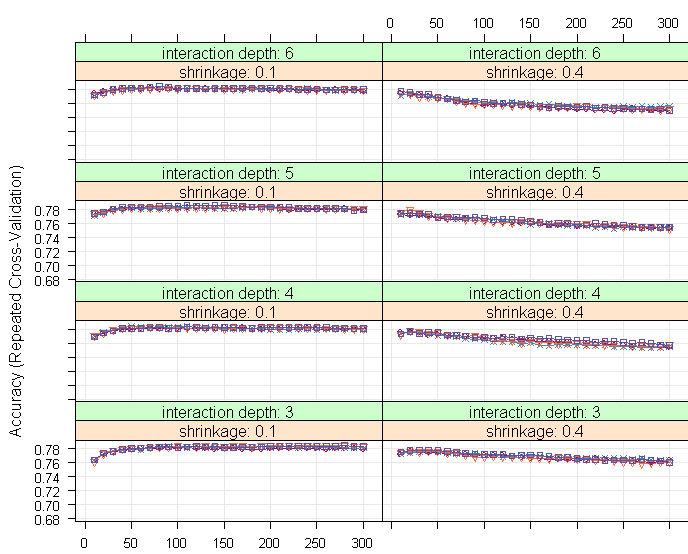
\includegraphics[scale=0.6]{figgbm.png}}
\caption{Performance of Gradient Boosted Trees}
\label{fig 1}
\end{figure}

Modeling influence using Decision trees with gradient boosting was performed. To tune the parameters of the trees such as Number of Trees $N_{trees}$, Shrinkage, Interaction depth and Minimum observations in nodes, a grid search was conducted. Training set Accuracy was the criteria to select the optimal model. Fig. 2 shows the performance of the algorithm during grid search and the accuracy is seen in Fig. 2 to degrade as the interaction depth increases beyond 5 and the shrinkage is increased beyond 0.1.  The final parameter values for the optimal model obtained through grid search were $N_{trees}$ = 110, interaction depth = 5, shrinkage = 0.1 and minimum observations in nodes = 20. The accuracy obtained on the test set was 0.8601.\\

Random forests (Rf) technique to model influence using the correlated features and removing correlation was performed. Advantage of random forests models are better accuracy but at the cost of interpret-ability of the model. The tuning parameter is Number of trees for these model whose value has to be determined empirically. The final model selected using training set accuracy had classification accuracy of 0.856 on the test set. The model with correlated features gave slightly better result 0.859. Removing correlation doesn’t improve accuracy on this dataset for the ANN and Rf.\\

Improving accuracy using ensembling, boosting or bagging at the cost of interpret-ability is a disadvantage for implementation. Such techniques have improved accuracy but such models obtained had more theoretical importance than practical value as seen in the NetFlix competition. Table V contains the training set and test set accuracy of greedy ensembles of GBM Trees, Random forests and ANN obtained in Section IV-B. The test set accuracy of the models is used as the selection criteria and Extreme Gradient Boosting has the highest accuracy on the test set at 0.87. ROC curves to denote the performance of Ensembled models of ANN, GBM, Rf is shown in Fig 3 and Area under curve is used as the selection criteria to obtain the optimal model. The results are shown for each combination in Fig. 3. The correlation between the predictions of GBM and Rf is 0.88 and so their ensemble was discarded due to highly correlated predictions. The highest accuracy on the test set is seen for the ensemble of GBM and Rf as shown in Table V.  \\

\begin{table}[!h]
\renewcommand{\arraystretch}{2.5}
\caption{Ensembled Predictors}
\label{table}
\centering
\begin{tabular}{|c|c|c|c|}
  \hline
\multicolumn{1}{|c|}{\textbf{Sr. No}} & \multicolumn{1}{c|}{\textbf{Technique}} & \multicolumn{1}{c|}{\textbf{Training Accuracy}} & \multicolumn{1}{c|}{\textbf{Test set Accuracy}}\\
  \hline
  1 & Boosting &  0.7856 & 0.82 \\
  \hline
  2 & Greedy Ensemble (ANN,GBM,RF) &  0.86 & 0.867 \\
  \hline
  3 & Greedy Ensemble (GBM,RF) &  0.86 & 0.83 \\
    \hline
  4 & Averaging Predictors (GBM,RF) &  0.79 & 0.866 \\
    \hline
  5 & Extreme Gradient Boosting &  0.79 & 0.87 \\
  \hline
\end{tabular}
\end{table}






\begin{figure}[H]
\centering
\fbox{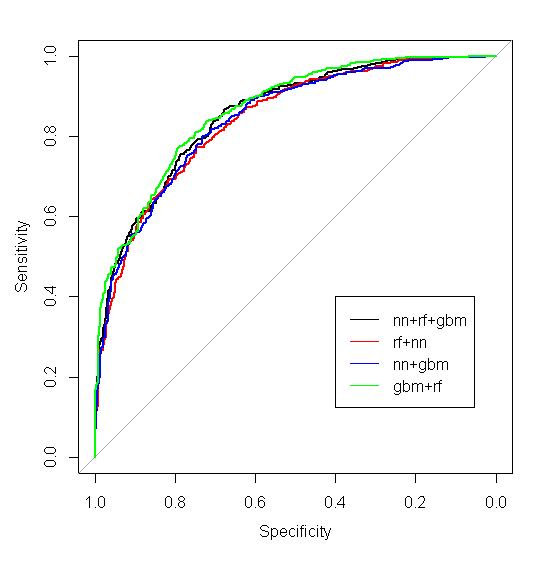
\includegraphics[scale=0.45]{figavg.png}}
\caption{Performance of Greedy Ensembles}
\label{fig 1}
\end{figure}



\section{Conclusion}
The framework for ranking influential nodes in a social network based on characteristics obtained from a nodes interaction on the social network has been presented in this paper. The influence is modeled using machine learning techniques unlike the conventional influence maximization approaches. Features of the individual nodes obtained from its interaction characteristics  are used and the network architecture is not considered. The performance metrics of the algorithms used in the experiments is classification accuracy and using this objective criteria Extreme Gradient Boosted decision tree has shown the highest accuracy. The influence ranking algorithm in this paper is a suitable technique for computation of the influence score of various nodes and this has been validated by the extensive experiments performed on Twitter dataset.  








\chapter{A Comparative Analysis of Community Detection Algorithms on Social Networks}



\section{Introduction}
% no \IEEEPARstart

\indent  Networks are used to graphically represent relationship or structure in many complex systems which can be seen in natural, technological or social settings. Understanding the process of formation of such networks or studying why certain systems exhibit a particular structure can provide insights into various phenomena that are commonly seen in real life communities such as diffusion, contagion and influence. These reasons have given birth to the scientific study of networks which became a multi disciplinary field spanning physics, computer science as well as social sciences \cite{aps:1} \cite{aps:2}. One reason for this occurrence is that any system in these fields can be represented in the form of a Network, a second reason is that the theories for studying such Networks have been at the intersection of all these fields \cite{aps:24}. Structurally a network or graph consists of nodes (vertices) and edges. An edge connects typically two nodes but if three or more nodes are connected by a single edge then such an edge is known as a hyperedge and such graphs are called hypergraphs. Other common networks seen in the world are scientific collaboration networks, where the nodes are the researchers and edges between them denote that they are working on the same research topic. An additional example is the Internet which in itself is a massive web graph consisting of web pages (nodes) and hyperlinks (edges). So it is concluded that in general any system can be represented as a network E.g citation networks, social networks, protein communities etc \cite{aps:24}. \\

Most networks of interest demonstrate community structures i.e. nodes (vertices) in them form a dense subgraph. Such subgraphs are referred to as clusters, modules or communities and they exhibit a degree of autonomy in the network\cite{aps:1}. These regions are called autonomous as the nodes in them interact frequently with other nodes in the same clusters than with nodes outside the clusters. Thus, such clusters correspond to entities that interact regularly to perform a function such as hormones responsible for producing an effect in the body or sensors in a home automation system responsible for detecting human presence in a room etc. Real world networks are so large that it is computationally infeasible to develop techniques for their study so in practise, methods are used that can simplify the structure of these large networks before any useful information can be extracted from them. These methods are known as Community Detection algorithms. There are over 100 algorithms that have proliferated in the network literature \cite{aps:10} \cite{aps:8}. The task of identifying communities is important as it offers insight into how a network is organised. This is because individual communities are functional units of the system and they help in understanding the role of the system. \\

The vertices in the network can also be classified on the basis of their roles they play with respect to the communities that they are a part of \cite{aps:24}. A central location makes the nodes important for diffusion of information within the network and so such nodes represent figures of importance with respect to that community. Similarly, the nodes that are located at the boundaries of a community might be acting as brokers for passing information to other communities and possibly play an important role in constraining the dynamics of spreading processes that occur on the network \cite{aps:10}. Other important reasons for creating coarse grain descriptions of networks are that using them missing information can be inferred about nodes by referring to the other nodes in its community or false information can be identified such as presence of an attribute that is uncommon in that community \cite{aps:10} \cite{aps:8}.
\\


Community detection of graphs is however an ill defined problem due to the absence of a universal definition of the object for detection i.e. "community". This has created multiple definitions for Communities, Methods to detect them and Performance evaluation techniques. Due to this ambiguity there is a diffusion of questionable literature in the domain of Network Science. Scientific opinion has changed its perception about networks. In the classical theory, clusters were viewed as dense sub graphs which exhibit a degree of autonomy in the network due to the presence of high edge density between nodes within the cluster than with nodes outside of it. Thus, the classical view relied more on the degree distributions of the nodes in the graph to determine clusters. This created ideas of strong communities and weak communities in a network that depended on the relation between the internal and external degree of the vertices of the graph \cite{aps:27}. The modern view relies more on calculating the probability of edge formation between nodes i.e. the community should be one in which there is a preferential linking pattern. This definition states that nodes in a community would have a higher probability of linking with each other than with nodes of other communities. Another approach that has developed used the link topology of the network and the trajectory of a random walker. The basis of this theory is that a random walk on the network would be concentrated for a longer interval in a dense sub-graph that corresponds to a community. This is because links moving out of a community would be supposedly lesser than those in it \cite{aps:28}. \\

In this paper, an evaluation of eight different state-of-the-art community detection algorithms available in the "igraph" package is performed. The package is a widely used collection of network analysis tools in R, Python, C and C++ and can be used on undirected and directed, weighted and unweighted graphs with overlapping or non overlapping communities. The graphs under examination are "Egonets" or egocentric networks of individuals obtained from Facebook. A review of the most widely used community detection algorithms is given in Section II followed by Experimental work in Section III and Conclusion in Section IV.


\section{Community Detection Algorithms}

\subsection{Walktrap - Computing communities in large networks using random walks}
The algorithm is based on the intuition that random walks on graphs are trapped into a dense part of the graph and such dense sub-graphs corresponds to communities. Walktrap is a agglomerative, hierarchical clustering algorithm that allows finding community structures at different scales. \\

The starting point is an initial partition $P_1$ of the graph with $n$ communities corresponding to the $n$ vertices of the graph i.e.   
Partition $P_1$ = $\lbrace\lbrace v \rbrace, v \epsilon V \rbrace$. A distance measure is used to compute vertex similarity between all adjacent vertices. Then the partition modifies itself by repeating the below operations at each step:\\

\begin{itemize}
\item For two adjacent communities $C_1$ and $C_2$ in $P_k$ merge into single community $C_3$ = $C_1$ $\cup$ $C_2$ and create a new partition $P_{k+1}$ = ($P_k$ : $\lbrace$ $C_1$ , $C_2$ $\rbrace$ ) $\cup \lbrace$ $C_3$ $\rbrace$ if it satisfies a criteria based on the distance between them, and
\item update distance between adjacent communities.\\
\end{itemize}

The algorithm at each step obtains a hierarchical data structure of communities called dendrogram. The algorithm computes the communities in time O(mnH) where n = $\mid V \mid$ vertices, m = $\mid E \mid$ edges and H = height of the dendrogram. For real world graphs which are sparse (m = O( log n)) it comes to O($n^2$ log n) \cite{aps:29}. The tunable parameters in this is the step size of the random walker $t$ which is used to calculate the probability that the random walkers shall move from a vertex $i$ to a vertex $j$. This probability is used to calculate the similarity between vertices and create clusters. The drawback of this method is that it is parameter dependent.\\ 

\subsection{Finding community structure in very large networks}
The "Fastgreedy" technique implemented in the paper has a running time of O($mHlog n$) on a graph with m = $\mid E \mid$ edges, n = $\mid V \mid$ vertices and h = height of the dendrogram \cite{aps:25}. In real world graphs which are sparse the computation time is linear O(n $log^2$ n). The algorithm is based on the greedy optimization of modularity and utilizes shortcuts in the optimization procedure of the original algorithm based on Greedy optimization of modularity \cite{aps:30} and efficient data structures to reduce the time complexity from O($n^2$) on sparse graphs to O(n $log^2$ n). Initially, every vertex belongs to a separate community, and communities are merged iteratively such that each merge is locally optimal. The algorithm stops when the modularity cannot be increased. It has lower time complexity than other techniques and its key drawback is that communities which have nodes and edges below a certain threshold are merged with adjacent communities. The algorithm has detected super communities in graphs that have no underlying clustering structure. It also relies on "modularity optimization" using approximation algorithms to reduce time complexity. However these have produced lower values of modularity than newer versions that have used Simulated Annealing to optimize modularity \cite{aps:33}.\\

\subsection{Finding and evaluating community structure in networks}
The "Edge-betweenness" is a hierarchical decomposition process where edges are removed in the decreasing order of their edge betweenness scores. This is motivated by the fact that edges connecting different communities have a higher probability to occur on the shortest paths between nodes of different communities. However the algorithm has a high running time of O($m^2$n). The repeated calculation of edge betweenness after an edge is removed has to be done for the entire graph. This affects the scalability of the algorithm to large graphs. At each iteration of this approach a full dendrogram is built and a measure to determine the optimal cut of the dendrogram can be made using modularity \cite{aps:31} \cite{aps:32}.  

\subsection{Near linear time algorithm to detect community structures in large-scale networks}
"Label Propagation algorithm" assign an initial unique label at random to the nodes of the network. Each label corresponds to a unique community to which the nodes belongs to. Then a particular node $n_1$ having 'k' neighbours determines it community affiliation based on the most frequent label amongst its neighbours. The problem however is that subgraphs in the
network that are bi-partite or nearly bi-partite in structure lead to oscillations of labels. Hence the label updation step is performed asynchronously. The stopping criteria of the iterative label assigning and re-assigning is till each node has a label to which maximum number of his neighbours belong to. Since the stopping criteria is not a measure to be maximised or minimised the algorithm has no unique solutions in heterogenous graphs with underlying community structure. The method has linear time complexity as every iteration is finished in O($m$) but yields different results based on the initial configuration (which has to be decided randomly), therefore one should run the method a large number of times and then build a consensus labeling, which could be tedious \cite{aps:34}. 

\subsection{Fast unfolding of communities in large networks}
"multilevel.community" is heuristic algorithm for obtaining communities from graphs by optimising the partition measure of modularity \cite{aps:35}. Modularity is the fraction of edges within a community substracted from expected fraction if edges were distributed at random. It is represented by Eqn 1. Since modularity optimization is NP-hard, an approximation algorithm is used that gives a running time of O($nlogn$). 

\begin{equation}
Q = \frac{1}{2m}\sum_{i,j}^{n} [A_{i,j} - \frac{k_i k_j}{2m} ] \delta (C_i C_j) 
\end{equation}

Where,
\begin{itemize}
\item $A_{ij}$ is edge weight between nodes i and j.
\item $k_i$ and $k_j$ are degrees of nodes i and j in case of unweighted graphs.
\item m is the sum of all edge weights in graphs
\item $c_i$ , $c_j$ are communities of nodes.
\item $\delta$ is 1 if edge exists between $c_i$ , $c_j$ and 0 otherwise;
\end{itemize}

The algorithm has two phases that are iteratively repeated:\\
Initially each nodes is assigned to its own unique community. Then for each node, the change in modularity is calculated by removing it from its community and moving it to the community of its neighbours. The change in modularity $\Delta Q$ is given by Eqn 2.

\begin{equation}
\Delta Q = [\frac{\sum_{in}^{}+2K_i,in}{2m} - (\frac{\sum_{tot} + k_i}{2m} )^2] - B
\end{equation}
\begin{equation}
B = [\frac{\sum_{in}^{}}{2m} - (\frac{\sum_{tot}^{}}{2m})^2 - (\frac{k_i}{2m})^2] 
\end{equation}

Where,
\begin{itemize}
\item $\sum_{in}$ is sum of all weights of links inside community to which $i$ is being assigned.
\item $\sum_{tot}$ is sum of all weights of links to nodes in community.
\item $k_i$ is weight degree of $i$
\item $k_i,in$ is the sum of the weights of links between $i$ and other nodes in the cluster.
\item $m$ is the sum of the weights of all links in the network
\end{itemize}

After calculation of $\Delta Q$ for all neighbour nodes of $i$, it is placed in the appropriate community that achieves local optima. This step is repeated for all nodes sequentially till each is assigned to its suitable community. In the second phase, the clusters formed after above step are treated as a single meta-node. The links within a cluster are treated as self loops to the cluster and the links in between clusters are represented as weighted edges between communities. The first pass is repeated again till all communities are organised in a hierarchy. This technique is most suitable for large graphs due to the low time complexity. However, the effects of the technique on the null benchmark i.e. Erdos Renyi random graphs is not verified. The technique is significant for detecting structure in overlapping clusters but not on graphs having non overlapping clusters.

\subsection{Statistical mechanics of community detection}
"spinglass.community" algorithm approaches the problem of community detection as finding the ground state of an infinite ranged Potts spin glass \cite{aps:36}. In this model, each vertex can be in one of $c$ spin states, and the interactions between the particles (i.e. the edges of the graph) specify which pairs of vertices would prefer to stay in the same spin state and which ones prefer to have different spin states. The model is then simulated for a given number of steps, and the spin states of the particles in the end define the communities. The tunable parameter of this technique is the upper limit for the number of clusters $c$ which make it supervised and not suitable for real world graphs. The algorithm is also non deterministic because of simulations needed. In sparse graphs the computational complexity of the algorithm is O($n^{3.2}$)

\subsection{Finding community structure in networks using the eigenvectors of matrices}
"leading.eigenvector.community" algorithm uses the concept of modularity maximization to obtain optimal partitions of the graph \cite{aps:36}. Due to the NP-hard nature of this problem, the modularity matrix is used for calculating the modularity. The eigenvalues and eigenvectors of the matrix are used for clustering. The largest eigenvalue is used to maximise the modularity of the network. This technique belongs to the spectral clustering techniques. This method has higher time complexity than the fast greedy method. Its computational complexity on sparse graphs is O($n^2$).

\subsection{Maps of random walks on complex networks reveal community structure}
"infomap.community" algorithm finds community structure that minimizes the expected description length of a random walker trajectory\cite{aps:36}. The algorithm is based on the Map Equation which yields the description length of an infinite random walk on a graph. The vertices are assigned unique codes and the random walk in the graph is described by the codes of the vertices it visited. Since each vertex has a unique code, the description can be lengthy. The description length can be reduced in a community structure by following the principles of geographic maps where vertices in different communities can have the same code. The best partition is the one that yields minimum description for the random walk.\\

The flow based methods provide different partitions than the methods based on structural features of the network like modularity. The results are striking in graphs having directed edges as these constrain the flow in the graph. The Map equation based techniques give importance to flow and are suitable for networks where structural features affect the dynamics of processes in the network like spread of epidemics, scientific collaborations etc. The runtime of the algorithm is $O(E)$       




% An example of a floating figure using the graphicx package.
% Note that \label must occur AFTER (or within) \caption.
% For figures, \caption should occur after the \includegraphics.
% Note that IEEEtran v1.7 and later has special internal code that
% is designed to preserve the operation of \label within \caption
% even when the captionsoff option is in effect. However, because
% of issues like this, it may be the safest practice to put all your
% \label just after \caption rather than within \caption{}.
%
% Reminder: the "draftcls" or "draftclsnofoot", not "draft", class
% option should be used if it is desired that the figures are to be
% displayed while in draft mode.
%
%\begin{figure}[!t]
%\centering
%\includegraphics[width=2.5in]{myfigure}
% where an .eps filename suffix will be assumed under latex, 
% and a .pdf suffix will be assumed for pdflatex; or what has been declared
% via \DeclareGraphicsExtensions.
%\caption{Simulation results for the network.}
%\label{fig_sim}
%\end{figure}

% Note that the IEEE typically puts floats only at the top, even when this
% results in a large percentage of a column being occupied by floats.


% An example of a double column floating figure using two subfigures.
% (The subfig.sty package must be loaded for this to work.)
% The subfigure \label commands are set within each subfloat command,
% and the \label for the overall figure must come after \caption.
% \hfil is used as a separator to get equal spacing.
% Watch out that the combined width of all the subfigures on a 
% line do not exceed the text width or a line break will occur.
%
%\begin{figure*}[!t]
%\centering
%\subfloat[Case I]{\includegraphics[width=2.5in]{box}%
%\label{fig_first_case}}
%\hfil
%\subfloat[Case II]{\includegraphics[width=2.5in]{box}%
%\label{fig_second_case}}
%\caption{Simulation results for the network.}
%\label{fig_sim}
%\end{figure*}
%
% Note that often IEEE papers with subfigures do not employ subfigure
% captions (using the optional argument to \subfloat[]), but instead will
% reference/describe all of them (a), (b), etc., within the main caption.
% Be aware that for subfig.sty to generate the (a), (b), etc., subfigure
% labels, the optional argument to \subfloat must be present. If a
% subcaption is not desired, just leave its contents blank,
% e.g., \subfloat[].


% An example of a floating table. Note that, for IEEE style tables, the
% \caption command should come BEFORE the table and, given that table
% captions serve much like titles, are usually capitalized except for words
% such as a, an, and, as, at, but, by, for, in, nor, of, on, or, the, to
% and up, which are usually not capitalized unless they are the first or
% last word of the caption. Table text will default to \footnotesize as
% the IEEE normally uses this smaller font for tables.
% The \label must come after \caption as always.
%
%\begin{table}[!t]
%% increase table row spacing, adjust to taste
%\renewcommand{\arraystretch}{1.3}
% if using array.sty, it might be a good idea to tweak the value of
% \extrarowheight as needed to properly center the text within the cells
%\caption{An Example of a Table}
%\label{table_example}
%\centering
%% Some packages, such as MDW tools, offer better commands for making tables
%% than the plain LaTeX2e tabular which is used here.
%\begin{tabular}{|c||c|}
%\hline
%One & Two\\
%\hline
%Three & Four\\
%\hline
%\end{tabular}
%\end{table}


% Note that the IEEE does not put floats in the very first column
% - or typically anywhere on the first page for that matter. Also,
% in-text middle ("here") positioning is typically not used, but it
% is allowed and encouraged for Computer Society conferences (but
% not Computer Society journals). Most IEEE journals/conferences use
% top floats exclusively. 
% Note that, LaTeX2e, unlike IEEE journals/conferences, places
% footnotes above bottom floats. This can be corrected via the
% \fnbelowfloat command of the stfloats package.

\section{Experiments}

The performance of the algorithms in Section II has been evaluated on the dataset provided in Section III (A)

\subsection{Dataset}

The testing of community detection algorithms is done on real or artificially generated networks where ground truth label for the communities is known as in the case of Zachary's karate club dataset or not known as in the case of GN bechmark or the LFR benchmark. The GN benchmark doesn't have the properties of a real network and so the LFR benchmark is used. In the LFR benchmark the vertex degree and community size are power law distributed as is seen in real world communities \cite{aps:26}. In this paper, in the evaluation of the algorithms "Egonets" of 60 user profiles obtained from Facebook are used. Egonets consist of a focal node "ego" and nodes to whom the ego is connected directly called "alters" along with ties between the alters. Such a network has hierarchical, overlapping communities along with homophilous strong ties. 


\begin{table}[!h]
\renewcommand{\arraystretch}{1.3}
\caption{Statistics of the Degree Distribution}
\label{table}
\centering
\begin{tabular}{|c|c|c|c|c|c|}
  \hline
\multicolumn{1}{|c|}{\textbf{Min}} & \multicolumn{1}{c|}{\textbf{I Quad.}} & \multicolumn{1}{c|}{\textbf{Median}} & \multicolumn{1}{c|}{\textbf{Mean}} & \multicolumn{1}{c|}{\textbf{III Quad.}} & \multicolumn{1}{c|}{\textbf{Max}}        \\
  \hline
  0 & 6 & 15 & 24.93 & 33 & 669\\
   \hline
\end{tabular}
\end{table}

\begin{table}[!h]
\renewcommand{\arraystretch}{1.3}
\caption{Statistics of the Order of the Egonets}
\label{table}
\centering
\begin{tabular}{|c|c|c|c|c|c|}
  \hline
\multicolumn{1}{|c|}{\textbf{Min}} & \multicolumn{1}{c|}{\textbf{I Quad.}} & \multicolumn{1}{c|}{\textbf{Median}} & \multicolumn{1}{c|}{\textbf{Mean}} & \multicolumn{1}{c|}{\textbf{III Quad.}} & \multicolumn{1}{c|}{\textbf{Max}}        \\
  \hline
  45 & 116.5 & 219 & 242 & 322 & 670\\
   \hline
\end{tabular}
\end{table}

Table I shows the statistics of the degree distribution obtained from all 60 egonets and Table II shows the summary statistics of number of the nodes of the 60 egonets. Fig 1 shows the histogram of degree distribution which resembles a power law distribution.

\begin{figure}[H]
\centering
\fbox{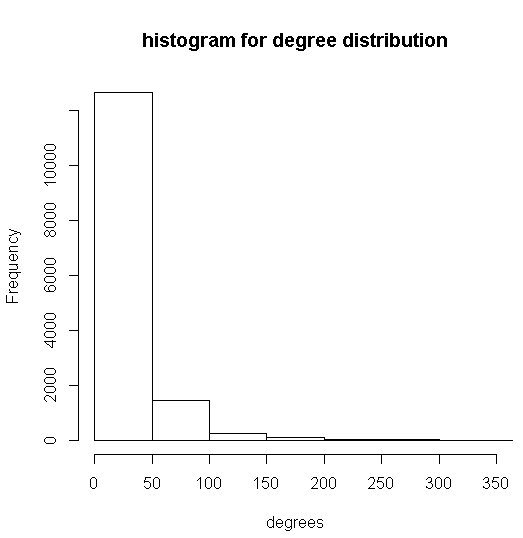
\includegraphics[scale=0.45]{histdeg.png}}
\caption{Histogram of Degree Distribution}
\label{fig 1}
\end{figure}

\subsection{Results}

Table III to X show the performance of the eight algorithms on the datasets. The results represent the modularity metric calculated on the optimal community structure generated on the dataset by the algorithms is given.

\begin{table}[!h]
\renewcommand{\arraystretch}{1.3}
\caption{Statistics of Performance of walktrap.community on Egonets}
\label{table}
\centering
\begin{tabular}{|c|c|c|c|c|c|}
  \hline
\multicolumn{1}{|c|}{\textbf{Min}} & \multicolumn{1}{c|}{\textbf{I Quad.}} & \multicolumn{1}{c|}{\textbf{Median}} & \multicolumn{1}{c|}{\textbf{Mean}} & \multicolumn{1}{c|}{\textbf{III Quad.}} & \multicolumn{1}{c|}{\textbf{Max}}        \\
  \hline
  0.04654 & 0.38017 & 0.50352 & 0.47555 & 0.58518 & 0.84149\\
   \hline
\end{tabular}
\end{table}

\begin{table}[!h]
\renewcommand{\arraystretch}{1.3}
\caption{Statistics of Performance of fastgreedy.community on Egonets}
\label{table}
\centering
\begin{tabular}{|c|c|c|c|c|c|}
  \hline
\multicolumn{1}{|c|}{\textbf{Min}} & \multicolumn{1}{c|}{\textbf{I Quad.}} & \multicolumn{1}{c|}{\textbf{Median}} & \multicolumn{1}{c|}{\textbf{Mean}} & \multicolumn{1}{c|}{\textbf{III Quad.}} & \multicolumn{1}{c|}{\textbf{Max}}        \\
  \hline
  0.2411 & 0.4220 & 0.4927 & 0.4960 & 0.5813 & 0.8299\\
   \hline
\end{tabular}
\end{table}

\begin{table}[!h]
\renewcommand{\arraystretch}{1.3}
\caption{Statistics of Performance of edge.betweeness.community on Egonets}
\label{table}
\centering
\begin{tabular}{|c|c|c|c|c|c|}
  \hline
\multicolumn{1}{|c|}{\textbf{Min}} & \multicolumn{1}{c|}{\textbf{I Quad.}} & \multicolumn{1}{c|}{\textbf{Median}} & \multicolumn{1}{c|}{\textbf{Mean}} & \multicolumn{1}{c|}{\textbf{III Quad.}} & \multicolumn{1}{c|}{\textbf{Max}}        \\
  \hline
  0.1566 & 0.3600 & 0.4896 & 0.4719 & 0.5921 & 0.8528\\
   \hline
\end{tabular}
\end{table}

\begin{table}[!h]
\renewcommand{\arraystretch}{1.3}
\caption{Statistics of Performance of label.propagation.community on Egonets}
\label{table}
\centering
\begin{tabular}{|c|c|c|c|c|c|}
  \hline
\multicolumn{1}{|c|}{\textbf{Min}} & \multicolumn{1}{c|}{\textbf{I Quad.}} & \multicolumn{1}{c|}{\textbf{Median}} & \multicolumn{1}{c|}{\textbf{Mean}} & \multicolumn{1}{c|}{\textbf{III Quad.}} & \multicolumn{1}{c|}{\textbf{Max}}        \\
  \hline
  0.0000 & 0.3323 & 0.4824 & 0.4469 & 0.5820 & 0.8482\\
   \hline
\end{tabular}
\end{table}

\begin{table}[!h]
\renewcommand{\arraystretch}{1.3}
\caption{Statistics of Performance of multilevel.community on Egonets}
\label{table}
\centering
\begin{tabular}{|c|c|c|c|c|c|}
  \hline
\multicolumn{1}{|c|}{\textbf{Min}} & \multicolumn{1}{c|}{\textbf{I Quad.}} & \multicolumn{1}{c|}{\textbf{Median}} & \multicolumn{1}{c|}{\textbf{Mean}} & \multicolumn{1}{c|}{\textbf{III Quad.}} & \multicolumn{1}{c|}{\textbf{Max}}        \\
  \hline
  0.2523 & 0.4546 & 0.5264 & 0.5205 & 0.6141 & 0.8557\\
   \hline
\end{tabular}
\end{table}

\begin{table}[!h]
\renewcommand{\arraystretch}{1.3}
\caption{Statistics of Performance of spinglass.community on Egonets}
\label{table}
\centering
\begin{tabular}{|c|c|c|c|c|c|}
  \hline
\multicolumn{1}{|c|}{\textbf{Min}} & \multicolumn{1}{c|}{\textbf{I Quad.}} & \multicolumn{1}{c|}{\textbf{Median}} & \multicolumn{1}{c|}{\textbf{Mean}} & \multicolumn{1}{c|}{\textbf{III Quad.}} & \multicolumn{1}{c|}{\textbf{Max}}        \\
  \hline
  0.2573 & 0.4379 & 0.4988 & 0.4908 & 0.5640 & 0.7188\\
   \hline
\end{tabular}
\end{table}

\begin{table}[!h]
\renewcommand{\arraystretch}{1.3}
\caption{Statistics of Performance of leading.eigenvector.community on Egonets}
\label{table}
\centering
\begin{tabular}{|c|c|c|c|c|c|}
  \hline
\multicolumn{1}{|c|}{\textbf{Min}} & \multicolumn{1}{c|}{\textbf{I Quad.}} & \multicolumn{1}{c|}{\textbf{Median}} & \multicolumn{1}{c|}{\textbf{Mean}} & \multicolumn{1}{c|}{\textbf{III Quad.}} & \multicolumn{1}{c|}{\textbf{Max}}        \\
  \hline
  0.2372 & 0.4250 & 0.5039 & 0.5050 & 0.6013 & 0.8321\\
   \hline
\end{tabular}
\end{table}

\begin{table}[H]
\renewcommand{\arraystretch}{1.3}
\caption{Statistics of Performance of infomap.community on Egonets}
\label{table}
\centering
\begin{tabular}{|c|c|c|c|c|c|}
  \hline
\multicolumn{1}{|c|}{\textbf{Min}} & \multicolumn{1}{c|}{\textbf{I Quad.}} & \multicolumn{1}{c|}{\textbf{Median}} & \multicolumn{1}{c|}{\textbf{Mean}} & \multicolumn{1}{c|}{\textbf{III Quad.}} & \multicolumn{1}{c|}{\textbf{Max}}        \\
  \hline
  0.04513 & 0.41261 & 0.50660 & 0.48933 & 0.60126 & 0.84931\\
   \hline
\end{tabular}
\end{table}

The highest mean modularity is obtained by the multilevel community detection algorithm. The real world datasets exhibit a community structure which might not be based on modularity. A second evaluation metric is used to calculate the edit distance between the ground truth communities in the dataset and the predicted communities by the algorithms.

\begin{table}[!h]
\renewcommand{\arraystretch}{1.3}
\caption{Running time of Algorithms on Egonets}
\label{table}
\centering
\begin{tabular}{|c|c|c|c|c|c|c|}
  \hline
\multicolumn{1}{|c|}{\textbf{Name}} & \multicolumn{1}{|c|}{\textbf{Min}} & \multicolumn{1}{c|}{\textbf{I Quad.}} & \multicolumn{1}{c|}{\textbf{Median}} & \multicolumn{1}{c|}{\textbf{Mean}} & \multicolumn{1}{c|}{\textbf{III Quad.}} & \multicolumn{1}{c|}{\textbf{Max}}        \\
  \hline
  EDG & 2583 & 4231 & 4641 & 5711 & 5519 & 11111\\
  \hline
  IMaP & 0.01 & 0.05 & 0.115 & 0.247 & 0.360 & 1.530\\
  \hline
  MLTL & 0.01 & 0.01 & 0.01 & 0.012 & 0.02 & 0.05\\
  \hline
  WLK & 0.00 & 0.01 & 0.02 & 0.046 & 0.052 & 0.47\\
  \hline
  FTG & 0.00 & 0.00 & 0.02 & 0.08 & 0.082 & 1.12\\
  \hline
  LDG & 0.00 & 0.04 & 0.09 & 0.14 & 0.152 & 1.96\\
  \hline
  LBP & 0.00 & 0.00 & 0.00 & 0.0048 & 0.01 & 0.02\\
  \hline
  SPG & 2.17 & 7.01 & 16.7 & 31.2 & 36.04 & 250.45\\
  
   \hline
\end{tabular}
\end{table}

Table XI shows the running time in millisecs needed by the algorithms on the dataset. The average nodes in the network were 242 with the minimum size of 45 and maximum of 670. The label propagation algorithm has obtained the lowest running time on the datasets. The highest time complexity is seen in the edge betweenness algorithm and it proves that it may not scale well to large datasets.

\subsection{Edit Distance metric}

Edit distance calculates the minimum number of edit operations needed for transformation of the predicted solution with the actual solution. Each of the following operations cost one edit: 
\begin{itemize}
\item Add user to an existing circle.
\item Remove user from a circle.
\item create a circle with one user.
\item delete a circle with one user.
\end{itemize}

\begin{table}[H]
\renewcommand{\arraystretch}{1.3}
\caption{Edit Distance of Algorithms on Egonets}
\label{table}
\centering
\begin{tabular}{|c|c|c|}
  \hline
\multicolumn{1}{|c|}{\textbf{Sr No.}} & \multicolumn{1}{|c|}{\textbf{Name}} & \multicolumn{1}{c|}{\textbf{Edit Distance}}  \\
  \hline
  1 & edge.betweenness & 14284\\
   \hline
  2 & multilevel & 15162\\
   \hline
  3 & infomap & 13988\\
   \hline
  4 & label.propagation & 14538\\
   \hline
  5 & spinglass & 15256\\
   \hline
  6 & fastgreedy & 14736\\
   \hline
  7 & walktrap & 14696\\
   \hline
  8 & leading.eigenvector & 15304\\
   \hline
\end{tabular}
\end{table}

From comparison of the edit distance metric shown in Table XII the infomap algorithm has obtained the lowest edit cost amongst the algorithms.



\section{Conclusion}
Egocentric networks present a challenge for community detection as the community structure in them is defined by the 'ego' to which the network belongs to. The presence of ground truth labels to the communities allows one to evaluate the precision of the algorithms effectively. The choice of algorithms therefore can be based on objective criteria like accuracy, running time and computational complexity. From our results, all algorithms with the exception of spinglass and edge betweenness were scalable and could be used on large networks. The partition quality is also an indicator of the accuracy of the algorithm, however real world datasets might not be based on optimum modularity. On this scale, the algorithms had mean modularity was close to each other. This was seen even in the case of algorithms like infomap and label propagation that don't partition based on optimum modularity. Finally, real world datasets exhibit heterogeneity due to which they may contain noise and also they do not have an fixed objective criteria for creation of communities. Therefore the edit distance measure showed high cost which meant that the partitions created by the algorithms had disagreements with the partitions made by the respective users or 'egos'.    


\chapter{Empirical Analysis of Data Clustering Algorithms}

\section{Introduction}
% no \IEEEPARstart
As the Digital transformation of the society gathers pace, there is an increase in proliferation of technologies that simplify the process of recording data efficiently. Low cost sensors, RFIDs , Internet enabled Point of Sales terminals are an example of such data capturing devices that have invaded our lives. The easy availability of such devices and the resultant simplification of operations due to them has generated repositories of data that previously didn't exist. Today, there exist many areas where voluminous amount of data gets generated every second and is processed and stored. Some of the common fields are social networks, sensor networks, cloud storages etc. The availability of data as well as the reduction in cost of computation power have jointly boosted the fields of machine learning, pattern recognition, statistical data analysis and in general data science.  \\

Even though such a volume provides huge opportunities to academia and industry it also represents problems for efficient analysis and retrieval \cite{aps:1} \cite{aps:3}. To mitigate the exponential time and space needed for such operations data is compacted into meaningful summaries i.e. Exploratory Data Analysis [E.D.A.] which shall eliminate the need for storing data. In unsupervised learning literature such summaries are equivalent to "clusters". E.D.A. helps in visualization and promotes better understanding of the data. It utilizes methods that are at the intersection of machine learning, pattern recognition and information retrieval. Cluster analysis is the main task performed in it.  \\

A Cluster in a data is defined objectively using dissimilarity measures such as edit distance, density in a euclidean or non euclidean data space, distance calculated using Minkowski measures, proximity measures or probability distributions. All measures concur that a threshold value should be set for grouping of objects in a cluster and objects which exceed such a threshold are dissimilar and should be separated from the cluster. Clustering gives a better representation of the data since all objects within a cluster have less variability in their attributes and they can be summarised efficiently. Clustering has found applications in other fields like estimating the missing values in data or identifying outliers in data \cite{aps:7}. 
\\


Clustering is thus a meta learning approach for getting insights into data and in diverse domains such as Market Research, E-Commerce, Social Network Analysis and Aggregation of Search Results amongst others. Multiple algorithms exist for organizing data into clusters however there is no universal solution to all problems. No consensus exists on the "best" algorithm as each is designed with certain assumptions and has its own biases. These algorithms can be grouped into methodologies such as Partitioning based, hierarchical, density based, grid based, message passing based, neural network based, probabilistic and generative model based. However in terms of complexity it is a NP-hard grouping problem and so existing algorithms rely on approximation techniques or heuristics to reduce the search space in order to find the optimal solution. There is no universally agreed objective criteria for correctness or clustering validity and each of these algorithms has its own drawbacks and successes in solving the challenging problem of unsupervised clustering \cite{aps:5} \cite{aps:4} . \\

Motivated by these reasons, in this paper a review of the state of the art clustering algorithms is made to highlight their main strengths and weaknesses. Section II covers the theoretical aspects of these algorithms, Section III contains the Experiments performed using these algorithms and Section IV has the conclusion on the results. 


\section{Types of Clustering Algorithms}

Various clustering algorithms are found in literature \cite{aps:2} \cite{aps:7} \cite{aps:3} \cite{aps:4} and are broadly categorized into categories on the basis of an algorithm designer's perspective with emphasis on the underlying clustering criteria:

\subsection{Partition based clustering algorithms}
 
The general principle in these algorithms is that a cluster should contain atleast one object and that each object must belong to exactly one group i.e. hard clustering. The Number of clusters $k$ is pre-specified by the user making this a semi supervised algorithm although many strategies have been suggested to estimate the ideal number of clusters like the empirical method where $k=\sqrt{n}$ where $ n$ = $\mid N \mid$ points and Elbow method where the $k$ is fixed as the turning point on the graph of $k$ v/s Avg. distance to centroid. The objective function to be minimised in these k-partitioning algorithms is $SSE$ i.e. Sum of Squared Distance \cite{aps:37}.

\begin{equation}
SSE = \sum_{k=1}^{k} \sum_{x_i \epsilon c_k} \left \| x_i - c_k \right \| ^2
\end{equation}

where $c_k$ = centroid of the cluster,\\

Popular k-partitioning algorithms are K-Means which represents a centroid as the arithmetic mean of the objects in the cluster \cite{aps:38}. The algorithm was the most popular in this category even though it had drawbacks as it could not find non convex shaped clusters or handle non numerical attributes in higher dimensions. The time complexity was O($kN$) making it suitable for large datasets, however the algorithm could theoretically take infinite iterations to converge and its mean based appraoch was sensitive to noisy data or data with outliers. Algorithms depending on Euclidean Distance measures suffer from the 'Curse of Dimensionality' due to distances being inflated in higher dimensions. K-Means++ by D. Arthur \textit{et. al} 2007 \cite{aps:39} provides an improvement over K-Means by initializing the seed cluster centroids at maximum distance from each other. This technique has provided better results compared to random initializations with multiple repeats. Mini Batch K-Means by D. Sculley \textit{et. al} \cite{aps:40} uses randomly sampled subsets of original data in each iteration of clustering. The approach improves computing time at the cost of slight reduction in accuracy compared to the Original K-Means algorithm.\\

To overcome the susceptibility to noise in mean based approaches, K-Mediods algorithm represented clusters by objects located near the centroids. Partitioning Around Mediods (PAM) \cite{aps:38} is the most popular approach for mediods based partitioning however it has a computational time complexity of O($k(n-k)^2$) and hence wouldn't scale well to large datasets. Modified version of PAM such as CLARA (PAM with sampling) \cite{aps:39} and CLARANS \cite{aps:40} were proposed. CLARA has a computation time complexity of O($ks^2 + k(n-k)$) and CLARANS has O($n^2$) and so both methods wouldn't be applicable to large sets of data. \\

Kernel K-Means involves converting the points from euclidean space to high dimension kernel space. The kernel choices can be based on Mercer's criteria. R.B.F. or Gaussian is the common choice considered. The advantage of Kernel K-Means over K-Means is in finding non convex clusters albeit at the cost of computational time. BFR algorithm \cite{aps:41} is implemented for detecting clusters in large datasets in a single pass over the data. The algorithm makes a strong assumption that clusters have objects that are normally distributed and due to this it can't find clusters at tilted angles to the axes or clusters of random shapes.      
 
\subsection{Hierarchical Clustering algorithms}

This category of algorithms have a completely unsupervised approach as they do not require the users to specify the number of clusters in advance. The algorithms in this category are of two types: Agglomerative Clustering (AGNES) and Divisive Clustering (DIANA). In Agglomerative, every object is treated as a cluster in the first pass and proximity based measures are used to determine which clusters can be merged in subsequent iterations. In divisive methods, a top down approach is followed in which all datapoints are merged in a single cluster initially and in subsequent iterations the supercluster is split into subclusters till a stopping criteria is reached. Computation time is the key drawback in such algorithms O($n^3$) / O($n^2 log n$) for priority queue implementations and so it is not applicable for large datasets which don't fit in main memory. Distance measures used are Cohesion ($d$ = diameter of a cluster i.e. maximum distance between points in a cluster), Radius ($r$ = maximum distance of a point from a cluster) or Density ($\frac{n}{d}$ ). \\

It is difficult to decide a distance measure for the data and hence the optimization objective isn't clear. Hierarchical clustering in general can't handle missing values except for probabilistic hierarchical methods and are sensitive to noise/outliers. The clusters once formed in an iteration cannot be undone in subsequent iterations. The result of clustering is a tree based data structure called dendrogram. In it the leaf nodes are the edges and clustering is indicated by joining leaf nodes by edges. To measure the dissimilarity between clusters several linkage methods are developed, the popular techniques are listed below. \\

\begin{itemize}
\item Maximum linkage clustering: max { d (a,b) : $a \in A, b \in B$}
\item Minimum linkage clustering: min { d (a,b) : $a \in A, b \in B$}
\item Average linkage clustering: $\frac{1}{|A||B|} \sum_{a \in A} \sum_{b \in B} d(a,b)$ 
\item Centroid linkage clustering: $||C_i - C_j||$ centroid $C_i \in A$ and centroid $C_j \in B$.
\item Ward's minimum variance method to minimize the within cluster variance. \\
\end{itemize}

Popular Algorithms of hierarchical clustering covered in the literature are BIRCH \cite{aps:42}, CURE \cite{aps:43}, ROCK \cite{aps:43}, CHAMELEON \cite{aps:44}. BIRCH is a scalable, hierarchical clustering approach for large datasets. It builds a Clustering Feature tree which is a height balanced tree. Similar to a B+ Tree it has leaf nodes that represent clusters by a tuple: {N,LS,SS} where $N$ is the number of points in the cluster, $LS$ is the linear sum of $N$ points and $SS$ is the squared sum of $N$ points. This creates compaction as individual data points are stored as summarised information. The non leaf nodes have atmost $B$ entries and leaf nodes have atmost $L$ subclusters that satisfy a threshold value for maximum radius. As new datapoints are assigned to nearest subclusters, the leaf nodes are split to remain under the threshold radius. A single pass is sufficient to cluster the data, however BIRCH is suitable only for numerical data and since each node in the CF Tree is limited by the size, the clusters formed may not be same as natural clusters. The algorithm doesn't perform well against non convex clusters as it uses radius to control the boundary of clusters.\\

CURE addresses the drawback of non-spherical shaped clusters. A constant number of $c$ well scattered points are chosen to represent the cluster. These points are shrunk towards the mean of the cluster by a fraction $\alpha$. Clusters with closest pair of representative points are merged at each iteration. ROCK is for large datasets with categorical attributes. It has a bottom up approach to clustering as initially each data point is a separate cluster. Then pairwise similarity is calculated by Eqn. 2 and a goodness function in Eqn. 3 is used to combine clusters. Calculation of pairwise similarity and merging clusters which are highly similar is done iteratively till a stopping criteria is reached. 

\begin{equation}
E_l = \sum_{i=1}^{k}n_i * \sum_{p_q,p_r \in C_k} \frac{link(p_q,p_r)}{n_i^{1+2f(\theta)}} 
\end{equation}

\begin{equation}
G(C_i,C_j) = \frac{link(C_i,C_j)}{(n_i+n_j)^{1+2f(\theta)} - (n_i)^{1+2f(\theta)} - (n_j)^{1+2f(\theta)}}  
\end{equation}  

CHAMELEON constructs a sparse graph from the dataset using K-nearest neighbour. It obtains clusters by partitioning the graph by minimising the edge cut. Individual clusters are merged based on relative inter-connectivity and relative closeness both overcoming disadvantage of BIRCH, CURE, ROCK as they merge based on a single criteria. However it has a high time complexity of O($nm + n log n + m^2log m$).


\subsection{Fuzzy clustering}

Fuzzy clustering algorithms assign a set of membership coefficients to each element which correspond to a "belongingness" or degree of membership to a cluster i.e. soft clustering. Fuzzy C-Means algorithm by Dunn in 1973 \cite{aps:45} and modified by Bezdek in 1981 \cite{aps:45} minimises the objective function in Eqn. 4 for this purpose, Eqn. 5 defines the degree of belongingness $u_{ij}^m$ and Eqn. 6 defines the centroid $C_j$ of a cluster.  

\begin{equation}
\sum_{j=1}^{k}\sum_{x_i \in C_j} u_{ij}^m (x_i - u_j)^2 
\end{equation}

Where,
\begin{itemize}
\item $u_{ij}$ is the degree to which an observation $x_i$ belongs to a cluster $C_j$
\item $μ_j$ is the center of the $C_j$
\item $m$ is the real number (1 $\leq m \leq \infty$) that defines the level of cluster fuzziness.

\end{itemize}

\begin{equation}
u_{ij}^m = \frac{1}{\sum_{l=1}^{k} (\frac{|x_i - c_j|}{|x_i - c_k|})^\frac{2}{m-1}}   
\end{equation}
\begin{equation}
C_j = \frac{ \sum_{x \in C_j} u_{ij}^m x}{\sum_{x \in C_j} u_{ij}^m}
\end{equation}
‏
The algorithm minimises intra cluster variance but can converge to a  local optimal solution. It depends on initialisation of the seeds and different initializations may lead to different results. The number of clusters $k$ have to be specified in advanced which is another drawback.

\subsection{Model Based Clustering Algorithms}

The traditional clustering algorithms hierarchical and partition based clustering rely on heuristics whereas Model based algorithms assume that the data has been generated from a mixture of multiple probability distributions (Gaussian or multinomial) whose parameters mean, covariance matrix are to be estimated using the Expectation Maximization algorithm. The Bayesian information criteria or the Akaike information criteria can be used for selection of optimal number of clusters. The key drawback of this algorithms is that similar to k-means it also can converge to local optimal solution depending on the initial assignment of the $k$ seeds. The objective function is not convex for these methods. Also, the optimization criteria can theoretically take infinite iterations to converge and a suitable threshold value has to be decided in advance. If the probabilities of the objects don't alter above this threshold then the algorithm can be stopped. Eqn. 6 is the prior probability that denotes the percentage of instances that came from source $c$. Eqn. 7 gives the mean i.e. expected value of attribute $j$ from source $c$. Eqn. 8 gives the covariance matrix denoting the covariance of attributes $j,k$ in source $c$.

\begin{equation}
P(c)= \frac{1}{n} \sum_{i=1}^{n} P(c\vert\vec{x_i})
\end{equation}
\begin{equation}
\mu_{c,j} = \sum_{i=1}^{n} \Bigl(\frac{P(c\vert\vec{x_i})}{nP(c)}\Bigr)x_{i,j}
\end{equation}
\begin{equation}
\sum_{c}{\mathstrut}_{j,k} = \sum_{i=1}^{n}\Bigl(\frac{P(c\vert\vec{x_i})}{nP(c)}\Bigr)(x_{i,j} - \mu_{c,j})(x_{i,k} - \mu_{c,k})
\end{equation}
\begin{equation}
 P(c\vert\vec{x_i}) = \frac{P(\vec{x_i}\vert c)P(c))}{\sum_{i=1}^{k}P(\vec{x_i}\vert c)P(c)}
 \end{equation}
 \begin{equation}
P(\vec{x_i}|c) = \frac{1}{\sqrt{2\pi\sum_{c}}} \exp\Bigl(- \frac{1}{2}(\vec{x_i} - \vec{\mu_c})^T \sum_{c}^{-1}(\vec{x_i} - \vec{\mu_c})\Bigr)
\end{equation}

\subsection{Grid Based Clustering Algorithm}  

The key principle of grid based algorithms is to discretize the dataspace into grids and estimate the density by counting the number of points in a grid cell. CLIQUE \cite{aps:3} \cite{aps:46} was developed by Agrawal \textit{et. al} to cluster high dimensional data in subspace. The algorithm identifies dense regions in a grid partition of the dataspace followed by selecting subspaces that contain clusters using Apriori principle. The dense connected units in all subspaces of interest are chosen and minimal cover for each cluster is created. However in all grid based clustering approaches the quality of clustering depends on the number and width of the grid cells. STING by Wang \textit{et. al} \cite{aps:46} divided the spatial area into rectangular cells at different levels of resolution forming a tree structure. A cell contain statistical parameters like mean, variance, standard deviations. This information is created by going through the data once and take O($n$) time to generate clusters. The algorithm doesn't consider the spatial relationship between neighbouring cells before a parent cell is constructed and so all cluster boundaries are horizontal or vertical but no diagonally shaped boundary is detected \cite{aps:46}.


\subsection{Density based clustering algorithms}

Cluster is defined as a connected dense component that can grow in any direction till the density continues to be above a threshold. This leads to automatic avoidance of outliers and detection of well separated clusters of arbitrary shapes. Popular methods based on this approach are DBSCAN by Kriegel \textit{et. al} \cite{aps:46}, OPTICS \cite{aps:46}. DBSCAN can find non linearly separable clusters and doesn't need the initial value of clusters to proceed. It uses euclidean distance measures to calculate distance between points in space and so is sensitive to curse of dimensionality. The parameters needed by DBSCAN are $\epsilon$ which defines the radius of neighbourhood around a point and minimum neighbours $MinPts$ of a point in its $\epsilon$ - neighbourhood. \\

In DBSCAN, pairwise distance is calculated between $x_i$ and other points. For each point in the $\epsilon$ - neighbourhood of $x_i$ if the $N_pts \leq MinPts$ then mark it as $core$ point. Then for each $core$ point create a new cluster or assign it to a cluster if it is not assigned already. Find recursively all its density connected points and assign them to the same cluster as the core point. Iterate through the remaining unvisited points in the dataset. At the end of all iterations, the unassigned points are outliers. \\

OPTICS is an extension of DBSCAN to address the drawback of detecting clusters in varying densities. It accepts the parameters of DBSCAN $\epsilon$ and $MinPts$ in neighbourhood $N_{\epsilon}(P)$. It additionally defines a new measure for every point known as $Core-Distance_{\epsilon, Minpts}(P) = C$ as in Eqn. 12 and $Reachability-Distance_{\epsilon, Minpts}(o,p) = R$ as in Eqn 13.\\

\begin{align}
C = \begin{cases}UNDEFINED; & if | N_{\epsilon(p)} | < MinPts\\smallest distance to N_{\epsilon}(p); & otherwise\end{cases}
\end{align}
\begin{align}
R = \begin{cases}UNDEFINED; & if |N_{\epsilon(p)}| < MinPts\\max(C, dist(o,p)); & otherwise\end{cases}
\end{align}

OPTICS produces a cluster ordering with respect to its density based clustering structure. 

\subsection{Affinity Propagation Clustering}

This technique is based on concept of message passing between data points \cite{aps:47}. It doesn't require the user to specify the number of clusters in advance. The initial input is a similarity matrix $s$ where $s(i,k)$ denotes suitability of point $k$ to be exemplar or representative of point $i$. and $s(k,k)$ is higher for points more preferred as exemplars. the value can be set to median to produce moderate number of clusters whereas too high can get many clusters and too low shall give less clusters.\\

Two kinds of messages are exchanged between the points "responsibility" $r(i,k)$ reflects suitability of point $k$ as an exemplar of $i$. The availability $a(i,k)$ denotes how appropriate it would be for $i$ to choose $k$ as its exemplar. Initially availability matrix is set to zero and the responsibilities for each point is calculate by the rule:

\begin{align}
r(i,k) \leftarrow s(i,k) - \max {a(i,k')+s(i,k')} : \forall k', k' \neq k
\end{align}

Then availability is updated by the rules:\\

\begin{align}
a(i,k)  \leftarrow \min \left( 0 , r(k,k) + \sum_{i'\notin {i,k}}  max(0,r(i'.k)) \right) for (i \neq k)\\
a(k,k) \leftarrow \sum_{i' \neq k} \max \left( 0, r(i',k)  \right)
\end{align}

The value of $k$ such that $a(i,k)+r(i,k)$ is maximum is selected as an exemplar for point $i$. The iterative updates for availability and responsibility matrices can be terminated after a limited iterations or after changes in the messages fall below a threshold. The time complexity is of the order O($N^2 T$), $N = samples$ and $T = iterations$ \cite{aps:48}.   

\subsection{Affiliation Graph Model} 

Community Affiliation graph model is a probabilistic generative model for the network \cite{aps:49} \cite{aps:53}. The assumption is that the network is generated by a model whose parameters have to be estimated. The model for a network with $V$ vertices, $C$ communities, $M$ memberships, $p_c$ probability associated with a community $c$ is represented by tuple $B(V,C,M,{p_c})$. Then the edge probability for each pair of node is computed by Eqn. 18

\begin{equation}
P(u,v) = 1 - \prod_{c \in M_u \cap M_v} (1 - p_c)
\end{equation} 
\begin{equation}
P(u,v) = 1 - exp(-F_u.F_v^T)
\end{equation} 
If $M_u \cap M_v = 0$ then P(u,v) = $\varepsilon$. $F_u$ is the vector that denotes the strengths of association of a node $u$ with each community in the network. The task is to find the matrix of memberships $F$ that maximises the likelihood of generating the graph. The log-likehood of this is Eqn. 19. The Gradient update algorithm is used to find the value of F as shown in Eqn. 20. 

\begin{equation}
l(F) = \sum_{u,v \in E} log(1 - \exp(-F_u.F_v^T)) - \sum_{u,v \notin E}(F_u.F_v^T)
\end{equation}
\begin{equation}
\bigtriangledown l(F_u) = \sum_{v \in N(u)} F_v \frac{\exp(-F_u.F_v^T)}{1 - \exp(-F_u.F_v^T)} - \sum_{v \notin N(u)} F_v
\end{equation}


\subsection{Spectral Clustering}

Spectral clustering outperforms k-means or single linkage and also has several advantages such as simple implementation. Spectral clustering can be solved by linear algebra methods \cite{aps:50}. The main tools for spectral clustering are graph laplacian matrices $L$. The fundamental concept is to partition a given similarity graph such that edges between different groups have low weights and edges within a group have high weights. \\
\begin{align}
L = D - A\\
L_{sym} = D^-1/2*L*D^-1/2\\
L_{rw} = D^-1*L
\end{align} 
Where,
\begin{itemize}
\item D = Degree matrix
\item A = Adjacency matrix\\
\end{itemize}
Spectral clustering popular examples are Unnormalised spectral clustering which uses $L$ and Normalised spectral clustering with $L_{sym}$ and $L_{rw}$. In both methods, the first $k$ eigenvectors $u_1,u_2,...,u_k$ corresponding to the $k$ smallest eigenvalues are computed to get matrix $U \in R^{n*k}$ which has $u_1,u_2,...,u_k$ as columns. Then for $y_i \in R^k$ which is the $i^{th}$ row of $U$, all rows are treated as points and clustered by k-means to get $k$ clusters. The normalised spectral clustering algorithms attempt to minimise inter cluster similarity and maximise intra cluster similarity whereas unnormalised spectral clustering attempts to minimise inter cluster similarity only. For computational simplicity $L_{rw}$ is used in clustering.   



% An example of a floating figure using the graphicx package.
% Note that \label must occur AFTER (or within) \caption.
% For figures, \caption should occur after the \includegraphics.
% Note that IEEEtran v1.7 and later has special internal code that
% is designed to preserve the operation of \label within \caption
% even when the captionsoff option is in effect. However, because
% of issues like this, it may be the safest practice to put all your
% \label just after \caption rather than within \caption{}.
%
% Reminder: the "draftcls" or "draftclsnofoot", not "draft", class
% option should be used if it is desired that the figures are to be
% displayed while in draft mode.
%
%\begin{figure}[!t]
%\centering
%\includegraphics[width=2.5in]{myfigure}
% where an .eps filename suffix will be assumed under latex, 
% and a .pdf suffix will be assumed for pdflatex; or what has been declared
% via \DeclareGraphicsExtensions.
%\caption{Simulation results for the network.}
%\label{fig_sim}
%\end{figure}

% Note that the IEEE typically puts floats only at the top, even when this
% results in a large percentage of a column being occupied by floats.


% An example of a double column floating figure using two subfigures.
% (The subfig.sty package must be loaded for this to work.)
% The subfigure \label commands are set within each subfloat command,
% and the \label for the overall figure must come after \caption.
% \hfil is used as a separator to get equal spacing.
% Watch out that the combined width of all the subfigures on a 
% line do not exceed the text width or a line break will occur.
%
%\begin{figure*}[!t]
%\centering
%\subfloat[Case I]{\includegraphics[width=2.5in]{box}%
%\label{fig_first_case}}
%\hfil
%\subfloat[Case II]{\includegraphics[width=2.5in]{box}%
%\label{fig_second_case}}
%\caption{Simulation results for the network.}
%\label{fig_sim}
%\end{figure*}
%
% Note that often IEEE papers with subfigures do not employ subfigure
% captions (using the optional argument to \subfloat[]), but instead will
% reference/describe all of them (a), (b), etc., within the main caption.
% Be aware that for subfig.sty to generate the (a), (b), etc., subfigure
% labels, the optional argument to \subfloat must be present. If a
% subcaption is not desired, just leave its contents blank,
% e.g., \subfloat[].


% An example of a floating table. Note that, for IEEE style tables, the
% \caption command should come BEFORE the table and, given that table
% captions serve much like titles, are usually capitalized except for words
% such as a, an, and, as, at, but, by, for, in, nor, of, on, or, the, to
% and up, which are usually not capitalized unless they are the first or
% last word of the caption. Table text will default to \footnotesize as
% the IEEE normally uses this smaller font for tables.
% The \label must come after \caption as always.
%
%\begin{table}[!t]
%% increase table row spacing, adjust to taste
%\renewcommand{\arraystretch}{1.3}
% if using array.sty, it might be a good idea to tweak the value of
% \extrarowheight as needed to properly center the text within the cells
%\caption{An Example of a Table}
%\label{table_example}
%\centering
%% Some packages, such as MDW tools, offer better commands for making tables
%% than the plain LaTeX2e tabular which is used here.
%\begin{tabular}{|c||c|}
%\hline
%One & Two\\
%\hline
%Three & Four\\
%\hline
%\end{tabular}
%\end{table}


% Note that the IEEE does not put floats in the very first column
% - or typically anywhere on the first page for that matter. Also,
% in-text middle ("here") positioning is typically not used, but it
% is allowed and encouraged for Computer Society conferences (but
% not Computer Society journals). Most IEEE journals/conferences use
% top floats exclusively. 
% Note that, LaTeX2e, unlike IEEE journals/conferences, places
% footnotes above bottom floats. This can be corrected via the
% \fnbelowfloat command of the stfloats package.

\section{Experiments}

Section II has examined custering algorithms from a theoretical point of view and in this section their performance on a clustering benchmark dataset is provided for an empirical evaluation.

\subsection{Dataset}

The Datasets selected are CURE-T2-4K and CLUTO-T8-8K which are publicly available artificially generated benchmarks by ClueMiner. The clusters can be identified by visualization but performance of clustering algorithms produces different results.




\begin{figure}[htbp]
\centering
\setlength{\lineskip}{\medskipamount}
\subcaptionbox{CURE-T2-4K\label{fig:1a}}{\includegraphics[width=0.5\textwidth]{cure.png}}\hfill
\subcaptionbox{CLUTO-T8-8K\label{fig:1b}}{\includegraphics[width=0.5\textwidth]{cluto.png}}
\caption{Artificial Benchmark Datasets for Clustering} \label{fig:1}
\end{figure}


\begin{table}[H]
\renewcommand{\arraystretch}{1.3}
\caption{description of Dataset}
\label{table}
\centering
\begin{tabular}{|c|c|c|c|}
  \hline
\multicolumn{1}{|c|}{\textbf{Name}} & \multicolumn{1}{c|}{\textbf{ Instances}} & \multicolumn{1}{c|}{\textbf{ Attributes}} & \multicolumn{1}{c|}{\textbf{ Classes}}  \\
  \hline
  CURE-T2-4K & 4200 & 3 & 7\\
   \hline
   CLUTO-T8-8K & 8000 & 3 & 9\\
    \hline
\end{tabular}
\end{table}

\subsection{Experimental Results}


\subsubsection{Partition based clustering Algorithm}

Results of K-Means in Fig 2, K-Means++ in Fig 3 and Kernel K-Means with RBF kernel in Fig 4 applied on the datasets shows the detection of clusters symmetric along the axes is better than irregular shaped clusters.

\begin{figure}[H]
\centering
\setlength{\lineskip}{\medskipamount}
\subcaptionbox{CURE-T2-4K\label{fig:1a}}{\includegraphics[width=0.5\textwidth]{cure-km.png}}\hfill
\subcaptionbox{CLUTO-T8-8K\label{fig:1b}}{\includegraphics[width=0.5\textwidth]{cluto-km.png}}
\caption{Clustering based on K-Means} \label{fig:1}
\end{figure}


\begin{figure}[H]
\centering
\setlength{\lineskip}{\medskipamount}
\subcaptionbox{CURE-T2-4K\label{fig:1a}}{\includegraphics[width=0.5\textwidth]{cure-kpp.png}}\hfill
\subcaptionbox{CLUTO-T8-8K\label{fig:1b}}{\includegraphics[width=0.5\textwidth]{cluto-kpp.png}}
\caption{Clustering based on K-Means++} \label{fig:1}
\end{figure}


\begin{figure}[H]
\centering
\setlength{\lineskip}{\medskipamount}
\subcaptionbox{CURE-T2-4K\label{fig:1a}}{\includegraphics[width=0.5\textwidth]{cure-kkmeans.png}}\hfill
\subcaptionbox{CLUTO-T8-8K\label{fig:1b}}{\includegraphics[width=0.5\textwidth]{cluto-kkm.png}}
\caption{Clustering based on Kernel K-Means} \label{fig:1}
\end{figure}



\subsubsection{Hierarchical clustering Algorithms}

Hierarchical clustering algorithms based on different cluster agglomeration methods were applied on the datasets. The methods were not able to separate the noise from the dataset. Another drawback of these techniques was inability to handle noise / outliers. The results show the merging of noisy data with the clusters. The single linkage method has resulted in a super cluster for both datasets as shown in Fig 5. In Fig 6. Average linkage method could not identify clusters of irregular shape. Agglomeration based on complete linkage has resulted in compact clusters as seen in Fig 7. Agglomeration based on centroid has been susceptible to noise as seen in Fig 8. as points not belonging to any cluster were included in clusters. Agglomeration based on Ward's minimum variance criteria too included noise points in the clusters and failed to identify irregular shaped clusters.      

\begin{figure}[H]
\centering
\setlength{\lineskip}{\medskipamount}
\subcaptionbox{CURE-T2-4K\label{fig:1a}}{\includegraphics[width=0.5\textwidth]{hclust-cure-sin.png}}\hfill
\subcaptionbox{CLUTO-T8-8K\label{fig:1b}}{\includegraphics[width=0.5\textwidth]{hclust-cluto-sin.png}}
\caption{Hierarchical Clustering based on Single linkage} \label{fig:1}
\end{figure}


\begin{figure}[H]
\centering
\setlength{\lineskip}{\medskipamount}
\subcaptionbox{CURE-T2-4K\label{fig:1a}}{\includegraphics[width=0.5\textwidth]{hclust-cure-avg.png}}\hfill
\subcaptionbox{CLUTO-T8-8K\label{fig:1b}}{\includegraphics[width=0.5\textwidth]{hclust-cluto-avg.png}}
\caption{Hierarchical Clustering based on Average linkage} \label{fig:1}
\end{figure}


\begin{figure}[H]
\centering
\setlength{\lineskip}{\medskipamount}
\subcaptionbox{CURE-T2-4K\label{fig:1a}}{\includegraphics[width=0.5\textwidth]{hclust-cure-com.png}}\hfill
\subcaptionbox{CLUTO-T8-8K\label{fig:1b}}{\includegraphics[width=0.5\textwidth]{hclust-cluto-comp.png}}
\caption{Hierarchical Clustering based on Complete linkage} \label{fig:1}
\end{figure}



\begin{figure}[H]
\centering
\setlength{\lineskip}{\medskipamount}
\subcaptionbox{CURE-T2-4K\label{fig:1a}}{\includegraphics[width=0.5\textwidth]{hclust-cure-cen.png}}\hfill
\subcaptionbox{CLUTO-T8-8K\label{fig:1b}}{\includegraphics[width=0.5\textwidth]{hclust-cluto-cent.png}}
\caption{Hierarchical Clustering based on Centroid linkage} \label{fig:1}
\end{figure}


\begin{figure}[H]
\centering
\setlength{\lineskip}{\medskipamount}
\subcaptionbox{CURE-T2-4K\label{fig:1a}}{\includegraphics[width=0.5\textwidth]{hclust-cure-ward-d.png}}\hfill
\subcaptionbox{CLUTO-T8-8K\label{fig:1b}}{\includegraphics[width=0.5\textwidth]{hclust-cluto-ward-d.png}}
\caption{Hierarchical Clustering based on Ward’s minimum variance method} \label{fig:1}
\end{figure}



\subsubsection{Fuzzy clustering Algorithm}
The number of clusters have to be specified in advance and the clustering overlap is controlled by the fuzzifier parameter $m$. Random initialization was done with multiple repeats to avoid convergence to local minima. The approach was sensitive to noise and clusters were symmetric around the axes. Irregular shaped clusters were not detected.

\begin{figure}[H]
\centering
\setlength{\lineskip}{\medskipamount}
\subcaptionbox{CURE-T2-4K\label{fig:1a}}{\includegraphics[width=0.5\textwidth]{fuzzy-cure.png}}\hfill
\subcaptionbox{CLUTO-T8-8K\label{fig:1b}}{\includegraphics[width=0.5\textwidth]{fuzzy-cluto.png}}
\caption{Fuzzy C-Means Clustering} \label{fig:1}
\end{figure}



\subsubsection{Model based clustering Algorithm}
Performance of the Model based clustering algorithm was evaluated on the datasets with the final model configuration selected by 10-cross fold cross validation. The initial seeds were randomly assigned 12 times to avoid local optima.

\begin{figure}[H]
\centering
\setlength{\lineskip}{\medskipamount}
\subcaptionbox{CURE-T2-4K\label{fig:1a}}{\includegraphics[width=0.5\textwidth]{cure-em.png}}\hfill
\subcaptionbox{CLUTO-T8-8K\label{fig:1b}}{\includegraphics[width=0.5\textwidth]{cluto-em.png}}
\caption{Clustering result of Model based clustering Algorithm} \label{fig:1}
\end{figure}




The mixture model based clustering has detected 8 clusters in CURE-T2-4K and 24 clusters in CLUTO-T8-8K as seen in Fig. 2 and incorrectly clustered instances were 50.23\% and 60.66\% respectively. A disadvantage of this approach was specification of the number of clusters initially.

\subsubsection{Density based Clustering Algorithms}

DBSCAN is parameter dependent and detected clusters of irregular shapes. It handled noise effectively. The key drawback is finding the right values of $\varepsilon$ and $MinPts$ for a particular dataset. The clusters having irregular densities and not well separated were merged in both datasets to give super clusters. OPTICS wasn't parameter sensitive and could identify clusters effectively.  

\begin{figure}[H]
\centering
\setlength{\lineskip}{\medskipamount}
\subcaptionbox{CURE-T2-4K\label{fig:1a}}{\includegraphics[width=0.5\textwidth]{cure-dbs.png}}\hfill
\subcaptionbox{CLUTO-T8-8K\label{fig:1b}}{\includegraphics[width=0.5\textwidth]{cluto-dbs.png}}
\caption{Clustering result of DBSCAN Algorithm} \label{fig:1}
\end{figure}



\begin{figure}[H]
\centering
\setlength{\lineskip}{\medskipamount}
\subcaptionbox{CURE-T2-4K\label{fig:1a}}{\includegraphics[width=0.5\textwidth]{cure-optics.png}}\hfill
\subcaptionbox{CLUTO-T8-8K\label{fig:1b}}{\includegraphics[width=0.5\textwidth]{cluto-optics.png}}
\caption{Clustering result of OPTICS Algorithm} \label{fig:1}
\end{figure}





\subsubsection{Affinity Propagation Clustering}

Advantage of Affinity propagation clustering is that number of clusters need not be specified in advance. The tunable parameter $q$ is input preference which can be interpreted as the tendency of a data sample to become an exemplar. Keeping the value minimum result in small number of clusters. In unsupervised setting, affinity propagation resulted in large number of clusters even with $q=0$. 

\begin{figure}[H]
\centering
\setlength{\lineskip}{\medskipamount}
\subcaptionbox{CURE-T2-4K\label{fig:1a}}{\includegraphics[width=0.4\textwidth]{cure-ap.png}}\hfill
\subcaptionbox{CLUTO-T8-8K\label{fig:1b}}{\includegraphics[width=0.4\textwidth]{cluto-ap.png}}
\caption{Unsupervised Affinity Propagation Algorithm} \label{fig:1}
\end{figure}


\begin{figure}[H]
\centering
\setlength{\lineskip}{\medskipamount}
\subcaptionbox{CURE-T2-4K\label{fig:1a}}{\includegraphics[width=0.4\textwidth]{cure-ap.png}}\hfill
\subcaptionbox{CLUTO-T8-8K\label{fig:1b}}{\includegraphics[width=0.4\textwidth]{cluto-ap.png}}
\caption{Supervised Affinity Propagation Algorithm} \label{fig:1}
\end{figure}



 

\subsubsection{Spectral Clustering}

The time complexity of spectral clustering is high O($n^3$) and so results on CLUTO-T8-8K could not be evaluated. On CURE-T2-4K dataset the algorithm could not identify clusters connected by a dense region. Noise points too were included in the clusters.  



\begin{figure}[H]
\centering
\includegraphics[scale=0.4]{cure-spec.png}
\caption{Spectral Clustering}
\label{fig 1}
\end{figure}

\subsection{Summary of Results}

\begin{table}[H]
\renewcommand{\arraystretch}{1.3}
\caption{Evaluation of clustering algorithms}
\label{table}
\centering
\begin{tabular}{|c|c|c|c|}
  \hline
\multicolumn{1}{|c|}{\textbf{Name}} & \multicolumn{1}{c|}{\textbf{ Time Complexity}} & \multicolumn{1}{c|}{\textbf{Parameters}} & \multicolumn{1}{c|}{\textbf{Detect Asym Clusters}}  \\
  \hline
  KMeans & O($nkd$) & 1 & No\\
  \hline
  KMeans++ & O($nkd$) & 1 & No\\
  \hline
  Kernel KMeans & O($nkd$) & 1 & No\\
  \hline
  Hierarchical clustering & O($n^2logn$) & 1 & No\\
  \hline
  Fuzzy CMeans & O($n$) & 2 & No\\
  \hline
  Model based & O($knp$) & 2 & No\\
  \hline
  DBSCAN & O($nlogn$) & 2 & Yes\\
  \hline
  OPTICS & O($nlogn$) & 2 & Yes\\
  \hline
  Affinity propagation & O($n^2T$) & 2 & No\\
  \hline
  Spectral clustering & O($n^3$) & 2 & No\\
 \hline
\end{tabular}
\end{table}

\section{Conclusion}
Cluster detection poses a challenge to algorithms especially when underlying model for formation of community structure is not available. This is the case in most real world situations and hence there is ambiguity regarding defining the term "cluster". Ideally the approach to clustering should not require user interference, however all the current clustering algorithms require parameter tuning and this could result in models that overfit the data and don't generalize well. The algorithms could not identify clusters in the benchmark datasets and had drawbacks like sensitivity to noise and outliers, high time and computational complexity and failure to detect clusters which were not well separated or of arbitrary shapes and densities.       










\chapter{Community Detection using Node Attributes: A Non-Negative Matrix Factorization Approach.}


\section{Introduction}
% no \IEEEPARstart
Exploratory Data Analysis [E.D.A.] is a domain on the
intersection of fields such as machine learning, pattern
recognition and information retrieval. The key goal of this
domain is to generate effective summarizations, visualizations,
information discovery and retrievals from data with a goal of reducing the exponential
costs involved in its storage. The main task performed in E.D.A. is
clustering analysis. Cluster analysis is a type of unsupervised
learning as cluster labels are not provided apriori or rather
are implicit in the data itself. The term "Cluster" doesn't have a
standard definition and hence there is subjectivity in the
deciding what forms a "Cluster". This has led to proliferation in the literature of clustering algorithms. Distance based definition of clusters have been explored
and have created a family of techniques such as partition
based clustering \cite{aps:3} , hierarchical clustering \cite{aps:4}, mixture
model based clustering \cite{aps:4}, fuzzy clustering \cite{aps:8} amongst
others. In contrast to a line of previous work a second
definition of clusters was proposed based on density, this
created popular algorithms such as DBSCAN, OPTICS \cite{aps:46}.\\

A related field is Community Detection which involves
identification of latent groups of entities in data. These groups
correspond to autonomous regions in the network which are known to have a higher
degree of homogeneity within its members than with members
of other groupings in the same network. In Network sciences such sub
groups are called communities and these are identified using
network topology. A vast area of literature has uncovered
several state of the art community detection algorithms that
aim to find such communities in un-directed as well as
directed graphs \cite{aps:2} . This literature is based
on concepts related to Information Theory or the trajectory of Random walks
on graphs or the Map Equation \cite{aps:10} \cite{aps:9}. Apart from
this, community detection also developed a concept called
modularity and a new family of algorithms were developed
that detected communities in graphs by optimizing modularity in a greedy manner \cite{aps:2} \cite{aps:8}.\\

Latent Dirichlet Allocation was another concept
that emerged and led to a new line of research on detecting
communities by utilizing meta-data that is associated with
the entities (nodes). This led to novel techniques that utilized the
information about network topology along with meta data
for obtaining generative models of networks \cite{aps:52} \cite{aps:51}. However even with such methods there
were drawbacks such as the limited applicability, as they
could not detect overlapping communities. A second drawback
is that they assumed soft node-community memberships, which
was not appropriate for modeling communities because they
did not allow a node to have high membership strength to
multiple communities simultaneously. Finally, such methods
had a large time complexity and couldn't be scaled to graphs
having more than 1000 nodes.\\

Non negative matrix factorization of the
term document matrix was found to be effective in document
clustering \cite{aps:56}. NMF was later extended to clustering by
aiming to learn the adjacency matrix of a graph. NMF
research did not pay attention to the interpretation of latent
factors which are used to find out the matrix. This led to
development of BIGCLAM which aimed to learn latent
factors which the authors argued represented strengths of
community affiliations of nodes. BIGCLAM and NMF both
used community affiliation knowledge of the nodes so that their membership strengths could be
estimated. While most existing literature \cite{aps:53}
focuses either on using the meta data or entity annotation for
improving the quality of community detection. \\

The paper is organized as follows. Section II briefly surveys
related work. In Section III, the statistical model of the
approach is defined, and in Section IV, the parameter fitting
procedure is provided in detail. This is followed by describing
experimental evaluation in Section V and the conclusion.\\

\section{Related Work}

Clustering approaches have their own biases in identifying
clusters in data but none is considered a universal
best fit. For example, the objective function to be minimized
in the k-partitioning algorithms is variance or $SSE$ i.e. Sum of Squared Distance. $  SSE = \sum_{k=1}^{k} \sum_{x_i \epsilon c_k} \left \| x_i - c_k \right \| ^2 $ where $c_k$ = centroid of the cluster. In this case the clusters are convex
but the optimization function converges to a local optima as the objective
function is non convex \cite{aps:2}. Hierarchical
Clustering algorithms are a category of algorithms
having a completely unsupervised approach to clustering.
They do not require the users to specify the number of clusters
in advance and are broadly of two types: Agglomerative
and divisive. To measure the dissimilarity between clusters
obtained in hierarchical clustering, linkage methods were
developed with several popular techniques being listed in the
literature \cite{aps:2} \cite{aps:8} \cite{aps:4}. But it difficult to decide on a suitable linkage method and at times the selection of a distance measure too isn't clear.\\

Fuzzy clustering (FCM) minimizes the objective function given as
$\sum_{j=1}^{k}\sum_{x_i \in C_j} u_{ij}^m (x_i - u_j)^2 $
 with $\mu$ being the fuzzifier and
$m$ defining the level of cluster fuzziness. The drawbacks seen in k-means such as non convex objective function, difficulty in detecting non linearly separable clusters etc. are also seen in FCM. The MST clustering
algorithm discussed in \cite{aps:54} is known to be capable of
detecting clusters with irregular boundaries. Unlike traditional
clustering algorithms, the MST clustering algorithm does
not assume a spherical shaped clustering structure of the
underlying data. If the
number of clusters $k$ is given in advance, the simplest way to
obtain $k$ clusters is to sort the edges of the minimum spanning
tree in descending order of their weights, and remove the
edges with the first $(k-1)$ heaviest weights. Undesired clustering
structures and an unnecessarily large number of clusters are
problems commonly faced by MST based clustering. \\


In \cite{aps:45} Mixture Model based clustering is discussed which
unlike the traditional clustering algorithms doesn't rely on
heuristics but assumes that the data has been generated from
a mixture of multiple probability distributions (Gaussian or
multinomial) whose parameters have
to be estimated. This is done using a technique called Expectation Maximization. Subspace clustering \cite{aps:2} \cite{aps:4} is based on key principle which
is to discretize the data-space into grids and estimate the
density by counting the number of points in a grid cell. Other
methods in the literature are Affinity propagation \cite{aps:3} which is based on concept of message passing, Spectral clustering \cite{aps:2}
in which the first $k$ eigenvectors $u_1,u_2,...,u_k$ corresponding to the $k$ smallest eigenvalues are computed to get matrix $U \in R^{n*k}$ which has $u_1,u_2,...,u_k$ as columns. Then for $y_i \in R^k$ which is the $i^{th}$ row of $U$, all rows are treated as points and clustered by k-means to get $k$ clusters. DB-SCAN,
OPTICS are based on the concept of density and treat clusters
are dense regions connected by less dense regions. However, none of this literature is applicable for clustering in networks.\\

Community detection is a field that deals with
obtaining coarse grained descriptions of large networks as real
world graphs are too large to be analyzed efficiently. 
This is done by utilizing network topology to detect communities
of nodes while ignoring node attributes. Topic Link LDA and Block LDA were the first to cluster graphs by jointly modeling links and node attributes. Topic
link LDA aims to quantify the effect of topic similarity
and community similarity to the formation of a link \cite{aps:52} \cite{aps:51}.
Block LDA is a joint model of two components, with one
that models links between pairs of entities represented as
edges in a graph with a block structure, and the second that
models text documents, through shared latent topics. There
has also been limited work on combining graph and content
information for community discovery leading to techniques
such as CESNA and BIGCLAM. CESNA was for statistically
modeling the interaction between the network structure
and the node attributes. The authors argued that this
would lead to more accurate community detection as well as
improved robustness in the presence of noise in the network
structure \cite{aps:53}. BIGCLAM is another approach that detects
both 2-mode as well as cohesive communities which may
overlap or be hierarchically nested and is based on affiliation
graph models.\\

To the best
our knowledge, in the research no mention could be found
of using the attributes of a data point for calculating the
latent features on the basis of which communities shall be
detected. The work in this paper is based on BIGCLAM framework but
the critical difference with existing techniques such as CESNA, AGMFIT and BIGCLAM is that attributes shall be used instead of community affiliations. The intuition here is that attributes are useful in determining the cluster affiliations and as such this intuition is also consistent with the phenomenon of "homophily" that is seen in human networks.\\




\section{Mathematical Model}
The stochastic generative model for generating communities
is presented in this section in which the probability of two
entities in data being present in the same community is
dependent on the attributes or the annotated text data
associated with these nodes. An efficient model fitting
procedure is the presented which allows for detecting
communities in the network. The current work is based on
the assumption that attributes of the data are categorical. The aim is to build upon BIGCLAM, an affiliation model for
community detection, however the objective is using attribute
information in place of affiliation information for building a bipartite graph which will be partitioned.\\

\textbf{Directed Attribute Affiliation Model:} BIGCLAM and AGMFIT are build on the Affiliation Graph Model based algorithms which use Maximum Likelihood Estimation to create a AGM from the network. Both however ignore importance of attributed of the nodes being responsible for community
creation. In Social networks, Homophily is the tendency to be associated with
others who share similar preferences and therefore attribute
associated with the entity in a network play an important
role in deciding communities. The hypothesis of correlation
between attributes and communities is reasonable as its
presence is also seen in empirical evidence provided in
the literature \cite{aps:53}. Based on this reasoning, a simple
conceptual model called Directed Attribute Affiliation Model
is formulated. This builds on the family of affiliation network
models, but in this work affiliation models are extended to
consider attributes.\\

To represent node and attribute affiliation a bipartite
affiliation graph is created where nodes are the bottom layer
and attributes to which they belong are shown as the top
layer as seen in Fig.\ref{fig 1}. A directed edge is created between an attribute and a node if the node has the attribute present in it. Such a bipartite graph can be constructed easily if attributes are binary valued. In case the attributes are continuous or categorical, a different mechanism might be needed. In this paper only binary attributes are considered. Cluster affiliation can then be modeled using such a
bipartite graph where directed edges are formed between
nodes and attributes to denote that those nodes contain
that attribute. \\

\begin{figure}[H]
\centering
\fbox{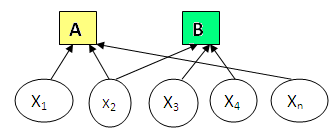
\includegraphics[scale=0.5]{bap.PNG}}
\caption{Bipartite Attribute Affiliation Graph}
\label{fig 1}
\end{figure}

A Bipartite Attribute Affiliation Graph is denoted as $B(X,C,M)$,
with $X$ as the nodes, $C$ as the attribute value and $M$ denotes
the directed edge from $X$ to $C$ if node $X$ has attribute
value $C$. The problem now is to create a set of communities
$S = S_1, S_2, ..., S_k$ given $B(X,C,M)$. A parameter $p_c$ is
assigned to an attribute value $c \in C$. This is for calculating
the probability that a node $x_i$ has the attribute value $c$. This
can also be called the probability that a node $x_i$ belongs to
the same community as another $x_j$ having the value of a
particular attribute as $c$. The $P_A(i, j)$ denotes that the nodes
$i, j$ belong to the same community $A$. This can be shown by
the below equation.

\begin{equation}
P_A(i,j) = 1 - \prod_{c \in M_i \cap M_j} (1 - p_c)
\end{equation} 

Where,

\begin{itemize}
\item $M_i$ = node $i$ has membership to attribute value $c$.
\item $M_j$ = node $j$ has membership to attribute value $c$.\\
\end{itemize}

In Eqn. 1, the value of $P_A(i, j)$ is set to $\varepsilon$, following
the BIGCLAM procedure the value of $\varepsilon$ can be set as
$2|E|/|V|(|V| - 1)$ [21].


\subsection{Calculate the latent weights of the attributes}

Every attribute has its own importance or strength in
determining the cluster to which the node should belong to,
this is denoted here formally as $F_{uC}$. This is the strength
that attribute $C$ has for node $u$ in determining its cluster.
Considering this membership strength the Eqn. 1 can be
modified as follows:

\begin{equation}
P_A(i,j) = 1 - exp(-F_{uC}.F_{vC}^T)
\end{equation}

$F_{uC}$ is the membership strength of a single attribute,
similarly it is assumed that every node $i$ has a attribute
membership vector $F_i$ which contains the membership
strengths to all attributes in the data. The modified probability
that nodes $i, j$ now share a cluster is Eqn 2.\\


The intuition behind the above formula is simple, Consider
a node having attribute values same as the attribute values
of another node, in such a case the likelihood of both
nodes belonging to a particular community increases. This
means that for each attribute a pair of nodes shares we
get an independent chance of grouping the nodes. Thus,
naturally, the more attributes a pair of nodes shares, the
higher the probability of sharing the same community and
being connected.\\


 
If $M_u \cap M_v = 0$ then $P(u,v) = \varepsilon$ this is done to consider
cases where nodes might not share attributes but still are
connected. $F_u$ is the vector that denotes the strengths of
association of a node $u$ with each attribute community in the network.
The task is to find the matrix of memberships $F$ that
maximizes the likelihood of generating the graph $G(V,E)$.
The log-likelihood of this is Eqn. 5. The Gradient update
algorithm is used to find the value of $F$ as shown in Eqn. 6 \\

\begin{equation}
l(F) = \sum_{u,v \in E} log(1 - \exp(-F_u.F_v^T)) - \sum_{u,v \notin E}(F_u.F_v^T)
\end{equation}
\begin{equation}
\bigtriangledown l(F_u) = \sum_{v \in N(u)} F_v \frac{\exp(-F_u.F_v^T)}{1 - \exp(-F_u.F_v^T)} - \sum_{v \notin N(u)} F_v
\end{equation}

\textbf{Decide Community Affiliation:} The membership strengths
matrix $F$ is computed from above and the next step is to
determine a suitable threshold above which it is possible to
determine whether the node $i$ belongs to a community. This
threshold is $\delta$ set at $\sqrt{−log(1 - \varepsilon)}$ [21]. The initialization
isn't done using locally minimal neighborhoods approach of
BIG-CLAM \cite{aps:53} as entity annotated attributes are used to get
initial values of the membership strengths $F_i$. The value of
$F_{i,k}$ is 0 if attribute $k$ is present and 0 if absent.\\

$\textbf{Choosing the number of communities:}$ This is done by
procedure specified in \cite{aps:53} where the model is trained using
an initial value of K. Then we detect K communities on the
80\% of node pairs and then evaluate the likelihood on the hold
out set. The K with the best hold out likelihood is used.\\

\section{Experiments}
In this section, evaluation of the performance of the variant of BIG-CLAM and other state-of-the-art community detection methods is done. The data-set used in this work consists of an artificially generated network with node attributes created using the tool described in the work of  Christine Largeron \textit{et. al.} \cite{aps:55}. Community detection methods such as Louvain and Fastgreedy technique were not applied as the graph was directed.

\subsection{Dataset and Evaluation Criteria}
The Artificially generated data-set is described below. The comparison metrics used are Variation of information (VI), Normalized mutual information, Split-join distance, Rand index (RI) and Adjusted Rand index (ARI). NMI, RI and ARI are in the range (0 - 1) with higher value indicating better clustering. The split-join distance between partitions A and B is the sum of the projection distance of A from B and the projection distance of B from A and should be low. VI should also ideally have a low value.

\begin{table}[H]
\renewcommand{\arraystretch}{1.3}
\caption{Description of the dataset}
\label{table}
\centering
\begin{tabular}{|c|c|c|}
  \hline
\multicolumn{1}{|c|}{\textbf{Sr. No}} & \multicolumn{1}{c|}{\textbf{Parameter}} & \multicolumn{1}{c|}{\textbf{Value}} \\
  \hline
  1 & Node Attributes &  3 \\
   \hline
  2 & Nodes &  200 \\
   \hline
  3 & Communities &  4 \\
   \hline
  4 & Observed homophily &  0.74 \\
   \hline
  5 & Modularity &  0.51 \\
   \hline
  6 & Avg. Clustering Coeff &  0.33 \\
   \hline
  7 & Avg. Degree &  5 \\
   \hline
  8 & Edges &  500 \\
   \hline
  9 & Network Type &  Directed-Unweighted \\
  \hline
\end{tabular}
\end{table}

\begin{figure}[H]
\centering
\fbox{\includegraphics[scale=0.5]{dataset.png}}
\caption{Artificially generated Network dataset}
\end{figure}

\subsection{Experimental Results}

\subsubsection{InfoMap}
"infomap.community" detected multiple communities in the network with few nodes leading to the conclusion that it split large clusters. The clustering is of poor quality as seen in Fig.\ref{InfoMap} as observed in the performance metrics.

\begin{table}[H]
\renewcommand{\arraystretch}{1.3}
\caption{Results}
\label{table}
\centering
\begin{tabular}{|c|c|c|}
  \hline
\multicolumn{1}{|c|}{\textbf{Sr. No}} & \multicolumn{1}{c|}{\textbf{Parameter}} & \multicolumn{1}{c|}{\textbf{Value}} \\
  \hline
  1 & Execution Time &  0.6 secs \\
   \hline
  2 & Modularity &  0.567 \\
   \hline
  3 & Variation of information &  1.72 \\
   \hline
  4 & Normalized mutual information &  0.565 \\
   \hline
  5 & Split-join distance &  115 \\
   \hline
  6 & Rand index &  0.717 \\
   \hline
  7 & Adjusted Rand index &  0.231 \\
  \hline
   8 & Detected Communities &  22 \\
  \hline
\end{tabular}
\end{table}

\subsubsection{Leading Eigenvector}
"leading.eigenvector.community" has uncovered a community structure with less communities as seen in Fig.\ref{leadg} and its performance is good on the metrics. 

\begin{table}[H]
\renewcommand{\arraystretch}{1.3}
\caption{Results}
\label{table}
\centering
\begin{tabular}{|c|c|c|}
  \hline
\multicolumn{1}{|c|}{\textbf{Sr. No}} & \multicolumn{1}{c|}{\textbf{Parameter}} & \multicolumn{1}{c|}{\textbf{Value}} \\
  \hline
  1 & Execution Time &  0.53 secs \\
   \hline
  2 & Modularity &  0.551 \\
   \hline
  3 & Variation of information &  0.88 \\
   \hline
  4 & Normalized mutual information &  0.67 \\
   \hline
  5 & Split-join distance &  74 \\
   \hline
  6 & Rand index &  0.795 \\
   \hline
  7 & Adjusted Rand index &  0.510 \\
  \hline
   8 & Detected Communities &  6 \\
  \hline
\end{tabular}
\end{table}

\subsubsection{Label Propagation}
"label.propagation.community" has detected low number of communities as seen in Fig.\ref{labelp}. Performance of this technique is better than other approaches. 

\begin{table}[H]
\renewcommand{\arraystretch}{1.3}
\caption{Results}
\label{table}
\centering
\begin{tabular}{|c|c|c|}
  \hline
\multicolumn{1}{|c|}{\textbf{Sr. No}} & \multicolumn{1}{c|}{\textbf{Parameter}} & \multicolumn{1}{c|}{\textbf{Value}} \\
  \hline
  1 & Execution Time &  0.06 secs \\
   \hline
  2 & Modularity &  0.545 \\
   \hline
  3 & Variation of information &  0.597 \\
   \hline
  4 & Normalized mutual information &  0.778 \\
   \hline
  5 & Split-join distance &  35 \\
   \hline
  6 & Rand index &  0.91 \\
   \hline
  7 & Adjusted Rand index &  0.81 \\
  \hline
   8 & Detected Communities &  8 \\
  \hline
\end{tabular}
\end{table}

\subsubsection{Walktrap}
"walktrap.community" uncovers a community structure with higher modularity as seen in Fig.\ref{walkt}. Large number of small communities have been created and so this technique has low values on the performance metrics. 

\begin{table}[H]
\renewcommand{\arraystretch}{1.3}
\caption{Results}
\label{table}
\centering
\begin{tabular}{|c|c|c|}
  \hline
\multicolumn{1}{|c|}{\textbf{Sr. No}} & \multicolumn{1}{c|}{\textbf{Parameter}} & \multicolumn{1}{c|}{\textbf{Value}} \\
  \hline
  1 & Execution Time &  0.11 secs \\
   \hline
  2 & Modularity &  0.579 \\
   \hline
  3 & Variation of information &  1.32 \\
   \hline
  4 & Normalized mutual information &  0.548 \\
   \hline
  5 & Split-join distance &  76 \\
   \hline
  6 & Rand index &  0.777 \\
   \hline
  7 & Adjusted Rand index &  0.446 \\
  \hline
   8 & Detected Communities &  15 \\
  \hline
\end{tabular}
\end{table}

\subsubsection{Spinglass and Clique Percolation}
"spinglass.community" detects high number of communities and has low values on VI, Split join and ARI metrics. Hence clustering quality is low as seen in Fig.\ref{sping}. Clique percolation with $k=3$ detected community structure given in as seen in Fig.\ref{cliquep} but 10\% of the nodes were unclassified.

\begin{table}[H]
\renewcommand{\arraystretch}{1.3}
\caption{Results}
\label{table}
\centering
\begin{tabular}{|c|c|c|}
  \hline
\multicolumn{1}{|c|}{\textbf{Sr. No}} & \multicolumn{1}{c|}{\textbf{Parameter}} & \multicolumn{1}{c|}{\textbf{Value}} \\
  \hline
  1 & Execution Time &  13.91 secs \\
   \hline
  2 & Modularity &  0.35 \\
   \hline
  3 & Variation of information &  1.12 \\
   \hline
  4 & Normalized mutual information &  0.638 \\
   \hline
  5 & Split-join distance &  94 \\
   \hline
  6 & Rand index &  0.772 \\
   \hline
  7 & Adjusted Rand index &  0.419 \\
  \hline
   8 & Detected Communities &  8 \\
  \hline
\end{tabular}
\end{table}

\subsection{Community Structures}
The figures below show the community structures uncovered by different approaches.

\begin{figure}[H]
  \begin{subfigure}[b]{0.3\linewidth}
    \includegraphics[width=\linewidth]{infomap.png}
    \caption{infomap}
    \label{InfoMap}
  \end{subfigure}
  \hfill %%
  \begin{subfigure}[b]{0.3\linewidth}
    \includegraphics[width=\linewidth]{leadg.png}
    \caption{Leading Eigenvector}
    \label{leadg}
  \end{subfigure}
\caption{Community structures in Network}
\end{figure}


\begin{figure}[H]
  \begin{subfigure}[b]{0.3\linewidth}
    \includegraphics[width=\linewidth]{labelp.png}
    \caption{Label propagation}
    \label{labelp}
  \end{subfigure}
  \hfill %%
  \begin{subfigure}[b]{0.3\linewidth}
    \includegraphics[width=\linewidth]{walkt.png}
    \caption{Walktrap}
    \label{walkt}
  \end{subfigure}
 \caption{Community structures in Network}
\end{figure}

\begin{figure}[H]
  \begin{subfigure}[b]{0.3\linewidth}
    \includegraphics[width=\linewidth]{sping.png}
    \caption{Spinglass}
    \label{sping}
  \end{subfigure}
  \hfill %%
  \begin{subfigure}[b]{0.3\linewidth}
    \includegraphics[width=\linewidth]{cliquep.png}
    \caption{Clique Percolation}
    \label{cliquep}
  \end{subfigure}
  \caption{Community structures in Network}
\end{figure}

\subsection{Variation of BIGCLAM}
With the above experimental results as baselines, the variation of BIGCLAM approach suggested in the paper was applied. The attributes were used to create a Bipartite graph as given by Jure Lescovec \textit{et. al} \cite{aps:53}, however the key difference was that the nodes were now having edges with the attributes. Network topology was thus ignored and BIGCLAM now used the Non negative matrix factorization to calculate the strength of memberships of the nodes to the attributes. These would be used to decide memberships of nodes to communities. As seen in Fig.\ref{bigc} the hold out set has highest likelihood at $k=6$. One advantage of this approach was large communities were formed and so it was inferred that splitting into smaller communities was avoided. As BIGCLAM is highly scalable, the network of $10^5$ nodes can be processed efficiently.

\begin{table}[H]
\renewcommand{\arraystretch}{1.3}
\caption{Results}
\label{table}
\centering
\begin{tabular}{|c|c|c|}
  \hline
\multicolumn{1}{|c|}{\textbf{Sr. No}} & \multicolumn{1}{c|}{\textbf{Parameter}} & \multicolumn{1}{c|}{\textbf{Value}} \\
  \hline
  1 & Execution Time &  8.51 secs \\
   \hline
  2 & Maximum likelihood Estimate &  -1070 \\
  \hline
   3 & Detected Communities &  6 \\
  \hline
\end{tabular}
\end{table}

\begin{figure}[H]
\centering
\fbox{\includegraphics[scale=0.3]{bigc.png}}
\caption{Clustering Structure using Variant of BIGCLAM}
\label{bigc}
\end{figure}



\section{Conclusion}
Community detection using a joint model of node attributes and network topology is a challenging task as additional information has to be factored while maintaining efficiency criteria. The model implemented in this paper uses Non negative matrix factorization on Bipartite Attribute Affiliation model for community detection. This approach allows for nodes to have high membership strengths simultaneously to various attribute communities. This allows for creating nested, overlapping and hierarchical communities in networks. The intuition behind this technique is that if the number of attributes shared by two nodes are high then the nodes have a higher probability of belonging to a single community. As this approach is relying on the optimization principle of BIGCLAM hence it is possible to state that this method can also be scaled to large networks efficiently.    


 

%\include{Chapter5/chapter5}
%\include{Chapter6/chapter6}
%\include{Chapter7/chapter7}
\include{Conclusions/conclusions}
\include{Publication/publication}
%\include{Ref/ref}
%
%\backmatter % book mode only
%\appendix
%\chapter{Appendix I: Quaternions}

There exists a correspondence between the orientation of a $ 3D $ object represented by a $ 3 \times 3 $ orthonormal matrix and unit quaternions in the group $ SO(3) $ \citep{Murray}. Quaternions give a global parametrization of $ SO(3) $, by using four numbers instead of three to represent a rotation. A quaternion is a vector quantity of the form,

  \[Q=q_{0} + q_{1}i + q_{2}j + q_{3}k  \ \ \ \ \ \ \ \  qi \in \R, i = 0, . . . , 3,\] 
                            
where, $ q_{0} $ is the scalar component of $ Q $ and $ \vec{q}= (q_{1}, q_{2}, q_{3}) $ is the vector component. A convenient notation is $ Q = (q_{0}, \vec{q}) $ with $ q_{0} \in \R $, $ \vec{q} \in \R^{3} $.
The set of quaternions Q is a 4-dimensional vector space over the reals and the unit quaternion form a group with respect to quaternion multiplication is a rotation group. Multiplication is distributive and associative, but not commutative.

For rotation through an angle $ \theta $ about the axis $ n $, the Euler parameters are defined as \citep{Hanson},
\begin{align*}
e_{0}&=\cos(\theta / 2) \ \ \ \ \ \ \ \ \ \ \ \ \ \ \ \ \ e_{2}=\cos \beta \cdot\sin (\theta / 2)\\
e_{1}&=\cos \alpha \cdot\sin (\theta / 2) \ \ \ \ \ \ \ \ \ e_{3}=\cos \gamma \cdot\sin (\theta / 2)
\end{align*}
where, $ \alpha, \beta $ and $ \gamma $ are the elementary rotations about any given random axis.

Given a rotation matrix $ R=exp\left(\hat{\omega}\theta \right) $, we define the associated unit quaternion as 
$ Q = \cos (\theta / 2) $,  $ \omega\sin (\theta / 2) $
where, $ \omega \in \R^{3} $ represents the unit axis of rotation and $ \theta \in \R^{3} $ represents the angle of rotation.
Given a unit quaternion $ Q = \left(q_{0}, \vec{q} \right) $, we can extract the corresponding rotation by setting,

\begin{center}
\ \ \ \ \ $\theta = 2\cos ^{-1} q_{0}, \ \ \ \ \ \ \ 
\omega = \left\lbrace
\begin{array}{ll}
\frac{\vec{q}}{\sin (\theta / 2)} & \mbox{if $ \theta \neq 0,$}\\
0 & \mbox{otherwise,}
\end{array}
\right.\
$
\end{center}

and  \[R = exp\left(\hat{\omega}\theta\right).\] 

It is observed that the components of the quaternion are Euler parameters. The Euler parameters have a geometrical meaning and thus the same holds for the components of the corresponding unit quaternion.

The Frenet 3D coordinate frame can be expressed in the form of quaternions. Assuming that the columns of the equation given below are the vectors $ [t_{i}, n_{i}, b_{i}] $ respectively, $ [q'(t)] $ can be written in the form,
\begin{eqnarray}
\left[ 
\begin{array}{c}
q_{o}'\\
q_{1}'\\
q_{2}'\\
q_{3}'
\end{array}
\right]=
\dfrac{v}{2} 
\left[
\begin{array}{cccc}
0 & -\tau & 0 & -\kappa \\
\tau & 0 & \kappa & 0 \\
0 & -\kappa & 0 & \tau \\
\kappa & 0 & -\tau & 0
\end{array}
\right] 
\cdot
\left[ 
\begin{array}{c}
q_{o}\\
q_{1}\\
q_{2}\\
q_{3}
\end{array}
\right] 
\label{13}
\end{eqnarray}
where $ v = \parallel \dot{c} \parallel $ and, 
\begin{align*}
q_{o}= \cos (\theta / 2) = \dfrac{1}{\sqrt{2}} & \sqrt{\cos \theta +1} = \dfrac{1}{2} \sqrt{Trace (R) +1} \\
q_{1}=& \dfrac{R_{32}-R_{23}}{4q_{0}} \\
q_{2}=& \dfrac{R_{13}-R_{31}}{4q_{0}} \\
q_{3}=& \dfrac{R_{21}-R_{12}}{4q_{0}}
\end{align*}

Key properties of equation \ref{13} are \citep{Hanson},
\begin{enumerate}
\item The matrix on the right hand side is antisymmetric, so that $ q(t) \cdot q'(t)=0 $ is preserved and all unit quaternions remain unit quaternions as they are.
\item Nine coupled equations with six orthonormality constraints are reduced to four coupled equations with a single constraint of unit length.
\end{enumerate}

From the above equation \ref{13}, the $ curvature $,
\begin{equation}
\kappa = - \left[\dfrac{2(q_{3}q'_{0}+q_{1}q'_{2})}{v(q_{1}^{2}+q_{3}^{2})} \right]
\label{14} 
\end{equation}
and the $ torsion $,
\begin{equation}
\tau = \dfrac{2q'_{2}+v\kappa q_{1}}{vq_{3}}
\label{15}
\end{equation}
can be extracted by the quaternion frame. The Frenet equations \ref{14} and \ref{15} may be integrated to generate a unique moving continuous frame along the protein backbone, for nonvanishing $ \kappa (t) $ with its space curve.

\section*{Motivation for using Quaternions}

\begin{enumerate}
\item It can be observed that the description of Euler angles and exponential co-ordinates suffers from the problem of $ \textit{singularity} $ in certain situations \citep{Hanson}. The extraction of parameters from any given rotational transformation matrix produces a singular case as the maps being many to one. While with the unit quaternion, extraction of unit quaternion from given rotational transformation being unique, there is no such case in which the inverse produces singularity. In quaternion space, the scalars, vectors, and quaternions are unified. Besides this, spatial vector can be expressed in quaternion space provides us with elegant properties for manipulating equations.



\item The quaternion frame summarizes nine matrix elements with six orthonormality constraints necessary to reduce the actual number of parameters of the frame to the three Euler angles. This forms a $ 3D $ orientation frame in terms of four quaternion frame variables with the single constraint of unit length that provides $ \textit{less computaional complexity} $.



\item The Frenet frame is periodic but not globally defined. As soon as the inflection points \citep{shuangwei} occur in the plane it is observed that the normal components of the Frenet frame switches sign instantly, while the quaternion frame has no such abrupt changes. The Frenet frame becomes undefined when the curvature $ \left(\kappa\right) $, vanishes along a straight line segment or at inflection point. It provides no such prescription to define a smooth transition from the frame coming and leaving the straight segment. The quaternion frame is comparatively $ \textit{smooth} $ throughout.
\end{enumerate}














% ------------------------------------------------------------------------

%%% Local Variables: 
%%% mode: latex
%%% TeX-master: "../thesis"
%%% End: 

%\chapter{Appendix II}


 ------------------------------------------------------------------------

%%% Local Variables: 
%% mode: latex
%% TeX-master: "../thesis"
%% End: 

\setcitestyle{numbers}
\bibliographystyle{plainnat}
%\bibliographystyle{Classes/CUEDbiblio}


%\bibliographystyle{Classes/jmb} % bibliography style

\renewcommand{\bibname}{References} % changes default name Bibliography to References
\bibliography{References/references} % References file 

%\bibliography{References/references} 
%\bibliographystyle{ieeetr}

%\includepdf[pages=-]{paper_imc1}
%\includepdf[angle=90]{certi_imc}
%\includepdf{IFAC_email}
%\includepdf[pages=-]{ifacconf.pdf}
%\includepdf{IEEE_Trans_acceptance}
%\includepdf[pages=-]{trans_smartgrid}
\end{document}
